%%%%%%%%%%%%%%%%%%%%%%%%%%%%%%%%%%%%%%%%%%%%%%%%%%%%%%%%%%%%%%%%%%%%%%%%%%%%%%%%
% Template for USENIX papers.
%
% History:
%
% - TEMPLATE for Usenix papers, specifically to meet requirements of
%   USENIX '05. originally a template for producing IEEE-format
%   articles using LaTeX. written by Matthew Ward, CS Department,
%   Worcester Polytechnic Institute. adapted by David Beazley for his
%   excellent SWIG paper in Proceedings, Tcl 96. turned into a
%   smartass generic template by De Clarke, with thanks to both the
%   above pioneers. Use at your own risk. Complaints to /dev/null.
%   Make it two column with no page numbering, default is 10 point.
%
% - Munged by Fred Douglis <douglis@research.att.com> 10/97 to
%   separate the .sty file from the LaTeX source template, so that
%   people can more easily include the .sty file into an existing
%   document. Also changed to more closely follow the style guidelines
%   as represented by the Word sample file.
%
% - Note that since 2010, USENIX does not require endnotes. If you
%   want foot of page notes, don't include the endnotes package in the
%   usepackage command, below.
% - This version uses the latex2e styles, not the very ancient 2.09
%   stuff.
%
% - Updated July 2018: Text block size changed from 6.5" to 7"
%
% - Updated Dec 2018 for ATC'19:
%
%   * Revised text to pass HotCRP's auto-formatting check, with
%     hotcrp.settings.submission_form.body_font_size=10pt, and
%     hotcrp.settings.submission_form.line_height=12pt
%
%   * Switched from \endnote-s to \footnote-s to match Usenix's policy.
%
%   * \section* => \begin{abstract} ... \end{abstract}
%
%   * Make template self-contained in terms of bibtex entires, to allow
%     this file to be compiled. (And changing refs style to 'plain'.)
%
%   * Make template self-contained in terms of figures, to
%     allow this file to be compiled. 
%
%   * Added packages for hyperref, embedding fonts, and improving
%     appearance.
%   
%   * Removed outdated text.
%
%%%%%%%%%%%%%%%%%%%%%%%%%%%%%%%%%%%%%%%%%%%%%%%%%%%%%%%%%%%%%%%%%%%%%%%%%%%%%%%%

\documentclass[letterpaper,twocolumn,10pt]{article}
\usepackage{usenix-2020-09}

% abstract.sty  adjustbox.sty  cleveref.sty    couriers.sty  filecontents.sty
%hyphenat.sty  SIunits.sty     subfigure.sty  trackchanges.sty  ulem.sty
%usenix-2020-09.sty  wrapfig.sty
% adjcalc.sty   breakurl.sty   collectbox.sty  etoolbox.sty  flushend.sty
%multirow.sty  subcaption.sty  titling.sty    trimclip.sty
%usenix2019_v3.sty  usenix.sty

% to be able to draw some self-contained figs
\usepackage{usenix}
\usepackage{graphics}
\usepackage{cleveref}
\usepackage{titling}
\usepackage{trackchanges}
\usepackage{subcaption}
%\usepackage{subfigure}
\usepackage{tikz}
\usepackage{amsmath}
%\usepackage{abstract}
\usepackage{adjcalc}
\usepackage{adjustbox}
\usepackage{breakurl}
\usepackage{collectbox}
\usepackage{couriers}
\usepackage{etoolbox}
%\usepackage{filecontents}
\usepackage{flushend}
\usepackage{hyphenat}
\usepackage{multirow}
\usepackage{SIunits}
%\usepackage{trimclip}
%\usepackage{ulem}
\usepackage{wrapfig}
\usepackage{float}
\usepackage{multirow}
\usepackage{xargs}     % Use more than one optional parameter in a new commands
\usepackage{xcolor}  % Coloured text etc.
% 
\usepackage{graphicx}
\usepackage{subcaption}
%\usepackage{mwe}
\usepackage{paralist}
\usepackage[]{todonotes}
\usepackage{cleveref}
\crefformat{section}{\S#2#1#3} 
\crefformat{subsection}{\S#2#1#3}
\crefformat{subsubsection}{\S#2#1#3}

%\usepackage[subtle]{savetrees}

% inlined bib file
% \usepackage{references}

%-------------------------------------------------------------------------------
\begin{document}
%-------------------------------------------------------------------------------
%don't want date printed
\date{}
% make title bold and 14 pt font (Latex default is non-bold, 16 pt)
\title{\Large \bf OS Joules : A Study of Energy Efficiency and Operating
Systems}

%for single author (just remove % characters)
%\author{
%{\rm Your N.\ Here}\\
%Your Institution
%\and
%{\rm Second Name}\\
%Second Institution
% copy the following lines to add more authors
% \and
% {\rm Name}\\
%Name Institution
%} % end author

\maketitle

%-------------------------------------------------------------------------------
\begin{abstract}
  Optimizing energy and performance in a OS is tricky because there is a wide array of mechanisms and policies that could both individually and collaboratively impact the entire system. In this paper, we present findings from a detailed study of four network-driven workloads to explore in a grid of different dynamics in order to demonstrate the impact of hardware tuning on a general purpose OS and a application specific library OS. We find when tuning a general purpose OS, one can achieve improvements up to 48\% in energy and performance, and when tuning the library OS, we demonstrate improvements up to 74\%. Moreover, we built infrastructure in both systems to collect detailed time series log data on every hardware interrupt of various hardware and software information. The results in this paper include data from tens of thousands of experiments, each with detailed logs. Using these logs, we are able to better explain energy and performance improvements as well as demonstrate how hardware tuning can have both interesting and profound impacts on different OSes and its design and implementation.
  
%-------------------------------------------------------------------------------
%------------------------------------------------------------------------------
\end{abstract}

\section{Introduction}
\label{sec:intro}

% single applicaiotn -> performance + power


%The hardware nodes of a cloud service provider are often each dedicated to running a single cloud service component~\cite{FB}.
As latency-critical tasks become ubiquitous across data centers,
deploying them on dedicated nodes is becoming a well studied and favored decision~\cite{ixcp, heracles, PerAppPower, twine}.
Typically, this dedication prevents latency violations that might be triggered
by the co-location of best-effort batch tasks.
One hopes that this dedicated nature (i.e. fixed role in the service using a fixed software stack) can be exploited to obtain the required performance (e.g. 99\% tail latency) while minimizing the energy used, a key concern given the increasingly constrained energy budgets in data centers~\cite{ixcp, SmoothOperator, Dynamo, oldi-study, oldi-pegasus, NLP-energy}.

%General purpose OSes such as Linux have been designed to support a range of user software as well as the concurrent execution of competing applications, thus, they have evolved to include support for dynamically adjusting various hardware settings on modern CPUs and network interface cards (NICs). Past researchers have demonstrated that dedicating a node to a single application can attain dramatic performance gains~\cite{ix,arrakis, exokernel,ebbrt,rumpkernel, unikernels, aliraza}, these results also suggest that one may be able to cater a node's hardware parameters to obtain higher efficiency than allowing the OS to dynamically adjust them.

%While researchers have proposed application specific OSes in the past, their optimizations have mainly focused on OS level changes targeting performance.

%However, dedicating a node to a single application suggests that one may be able to manually tune the node's hardware settings to magnifiy the impact of such tuning. While researchers have proposed such systems in the past, referred to as library OSes~\cite{ix,arrakis, exokernel,ebbrt} or unikernels~\cite{rumpkernel, unikernels, aliraza}, this 
%Dedicating a node to a single application suggests that one may be able to manually tune the node's hardware parameters to fixed values and obtain higher efficiency than allowing the OS to dynamically adjust them.  Furthermore, it is possible that the impact of hardware tuning can be magnified if one starts with an application specific OS that has been designed and implemented for running a single dedicated application. 

However, the performance and energy use of a system are complex emergent properties of the myriad of interactions between application software, operating systems, hardware, and offered loads.
Interestingly, when we take a careful look at overall system execution under different energy profiles, we see that the consequences of tuning energy and performance reach far beyond directly observable quantities and impact the interactions between the aforementioned system components in subtle ways.
There is a dizzying array of operating system mechanisms and policies one must consider that could both individually and collaboratively impact the performance and energy use of the system.
Rather than focusing on the design and implementation of these mechanisms and policies, we find that we need a greater understanding of their underlying impacts and dynamics on energy and performance.


%
% table of workloads
%
%\begin{table}[t]
%\centering
%\begin{tabular}{l|c|c|c}
%  Name & Scenarios & Nature & CPU\\
%  \hline
%  NetPIPE & {\small 64B,8KB,64KB,512KB} & CL & Low\\ \hline
%  NodeJS & na & CL & High \\ \hline
%  Memcached & 200K, 400K, 600K & OL & Low \\ \hline
%  Silo & 50K, 100K, 200K & OL & High \\ 
%\end{tabular}
%\caption{Workload configurations: NetPIPE and NodeJS are single thread, single connection, closed-loop (CL) workloads. Memcached and Memcached-silo are multiple core, multiple connection, open-loop (OL) workloads. The column {\em CPU} indicates application compute demand on each request.}
%\label{table:wrkcfgs}	
%\end{table}


%
% summary landscape plots
%
      \begin{figure*}[t]
        \centering
        \begin{subfigure}[b]{0.45\textwidth}
            \centering
            \caption[]%
            {{\small Netpipe 64 KB message}}  
            \vspace*{-0.3cm}
            %\hspace*{0.35cm}  
            \label{fig:netpipe64Kov}
            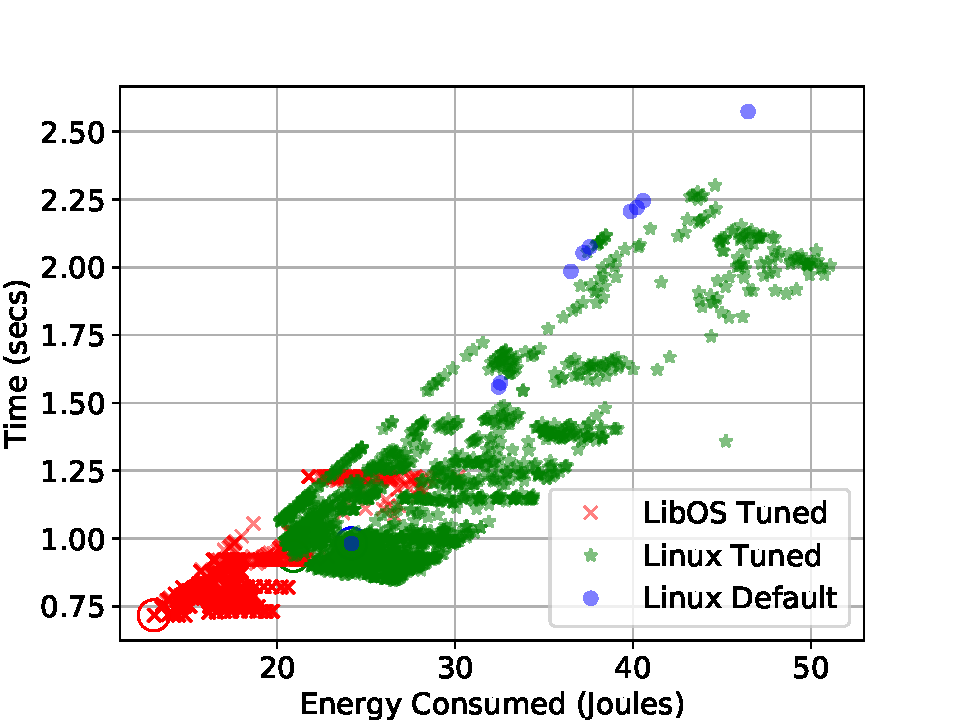
\includegraphics[width=\textwidth]{osdi_figures/netpipe_65536_overview.pdf}
        \end{subfigure}
%        \hfill
        \begin{subfigure}[b]{0.45\textwidth}  
            \centering 
            \caption[]%
            {{\small Memcached 600K QPS}} 
            \vspace*{-0.25cm}    
            \label{fig:mcdov}
            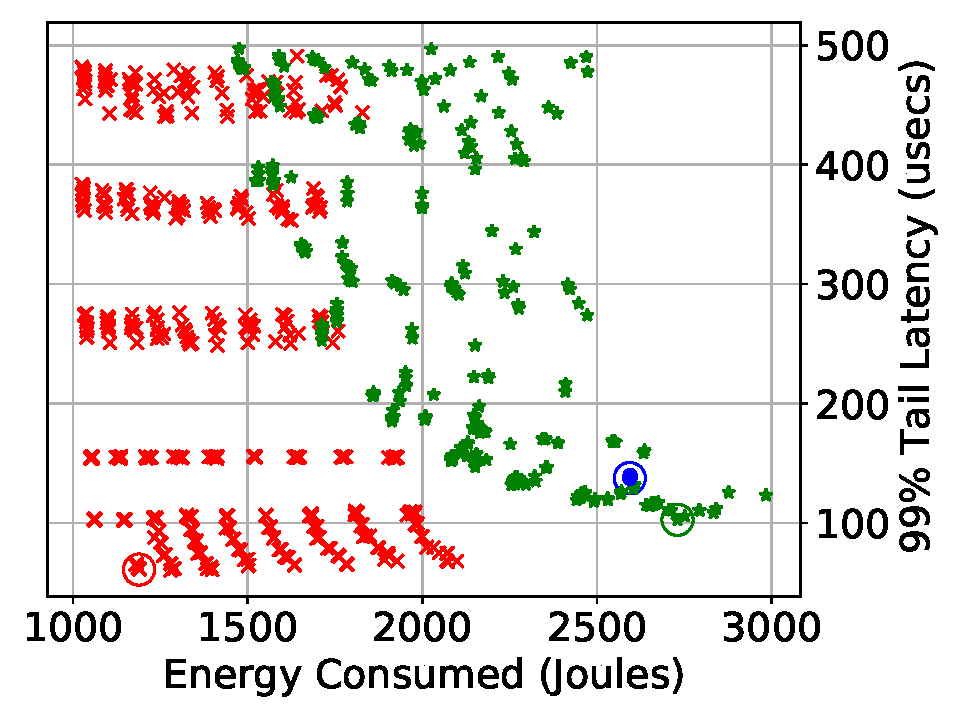
\includegraphics[width=\textwidth]{osdi_figures/mcd_600000_overview.pdf}
        \end{subfigure}
        \vskip\baselineskip
        \vspace*{-0.47cm} 
        \begin{subfigure}[b]{0.45\textwidth}   
            \centering 
            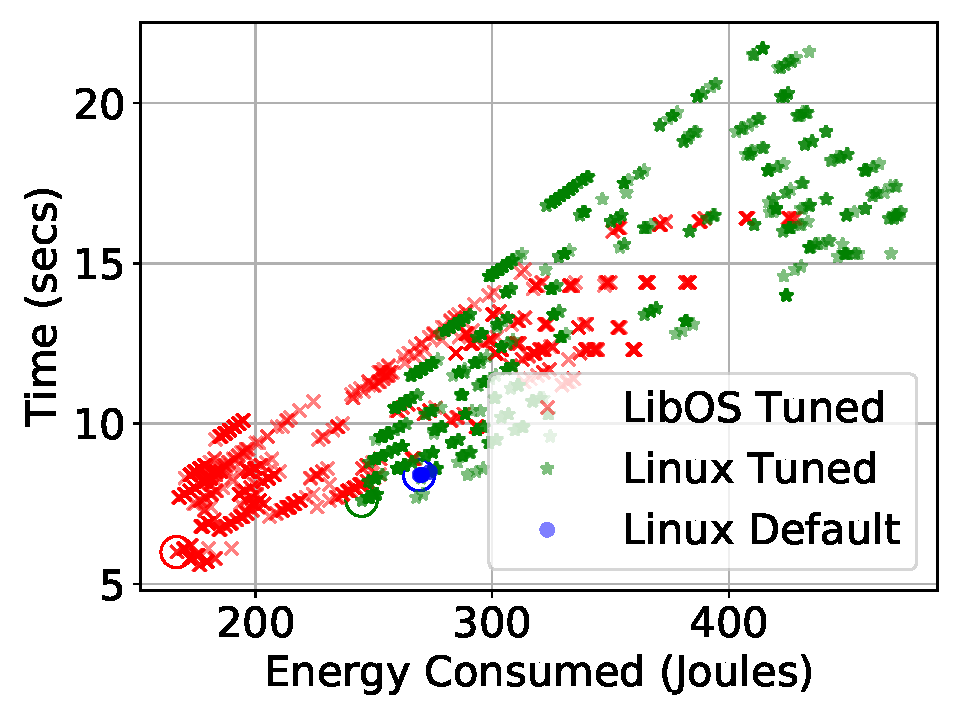
\includegraphics[width=\textwidth]{osdi_figures/nodejs_overview.pdf}
            \caption[]%
                    {{\small NodeJS 100K requests}}
                    %\hspace*{0.35cm}  
            \label{fig:nodejsov}
        \end{subfigure}
%        \hfill
        \begin{subfigure}[b]{0.45\textwidth}   
            \centering 
            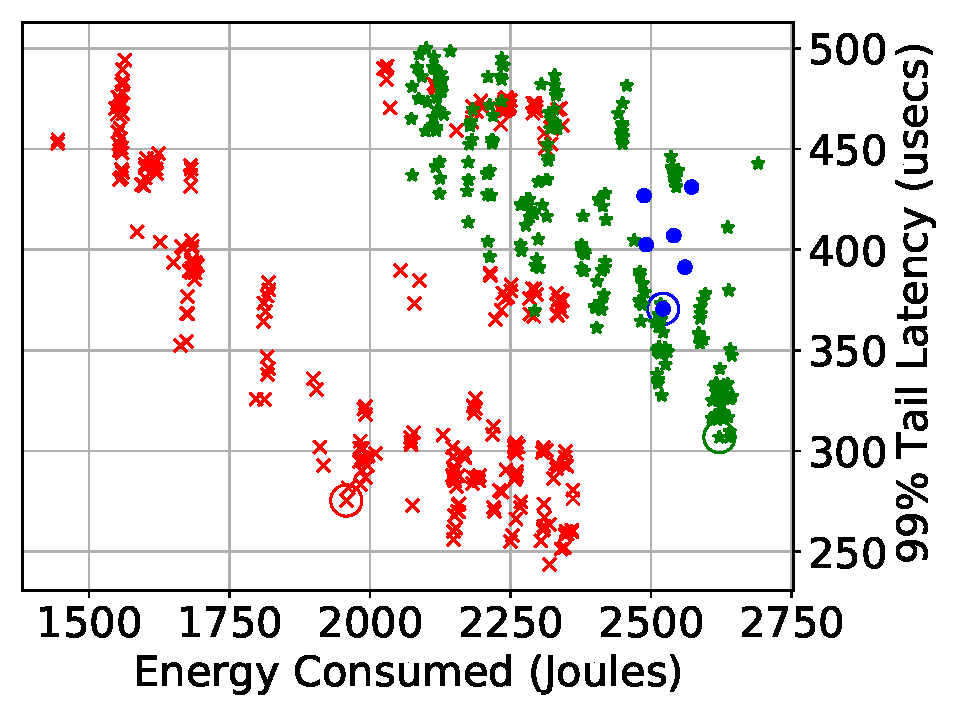
\includegraphics[width=\textwidth]{osdi_figures/mcdsilo_200000_overview.pdf}
            \caption[]%
            {{\small Memcached-silo 200K QPS}}    
            \label{fig:mcdsiloov}
        \end{subfigure}
        \caption[]
                {\small
These landscape plots portray the space of energy-performance profiles
that an OS/workload software stack can exhibit. The circle around individual points represent the min EPP values achieved in each workload.
\textit{Note that, in these plots, the origins do not start at zero
because the aim of the plots is to highlight structure within a plot
rather than to draw a comparison across plots.}
                  %Data from a run the settings associated with the 'best' EPP points are presented in~\ref{sec:data} and discussed in~\ref{sec:details}.          %Using these values we plot a timeline of the joule readings for one experimental run at the setting for Linux tuned and libOS along with data from a default Linux run of the workload.  The x-axis is the time offset from the beginning of the experiment.  For each log entry with a joule reading, we plot its value against its timestamp offset from the beginning of the run.  While the log has entries for every interrupt, we restrict sampling the joule counter to be at least 1ms apart as per the hardware manual's recommendation, as such not all log entries have an associated joule value.  To improve readability we only show a subset of the markers and use a line to connect the visible marks to the points not shown.    
        } 
        \label{fig:overview}
    \end{figure*}



%In this paper, we investigate the impact of hardware tuning on the performance and energy consumption of applications running on top of two baremetal OSes with fundamentally different design and implementation.
This study grew out of our efforts to explore a baremetal library OS for running datacenter workloads.
When configuring the library OS, we began by inheriting the default values that Linux uses on the same hardware.
However, it soon became clear that Linux's behaviour with respect to these settings was a complex mixture of dynamic and administrator controlled parameters.  
The actual impact and optimality of Linux's defaults on the energy consumption and realized application performance was not discernible though inspection and reasoning alone.
As a result, we decided to explore in detail the performance and energy use of both Linux and our library OS under a variety of hardware settings and workloads. 

We focus our study on three hardware settings - 1) Network Interface Card (NIC) Interrupt delay (ITR-delay), 2) Dynamic Voltage and Frequency Scaling (DVFS) and 3) Running Average Power Limit (RAPL) -
and four network-driven workloads (Table~\ref{table:wrkcfgs}) that span open and closed-loop dynamics with both low and high application CPU requirements. 
While open-loop latency-critical workloads tend to be common in the cloud, closed-loop workloads expose scenarios in which there is an interdependence between service performance and the offered load.
The range of closed-versus-open and high-versus-low CPU demand provides a rich ground for exposing and analyzing the behavior of the two target OSes.



%\subsection*{Summary of Findings}

We compare the performance of default Linux
running the workloads under the 11 scenarios in Table~\ref{table:wrkcfgs}
to that of {\em tuned} Linux and {\em tuned} library OS,
both configured across a wide range of static values
for the three hardware settings.   
We built infrastructure in both systems to collect detailed time series log data on every network interrupt (see Section \ref{sec:log_collect} for details).
This data includes a high-precision timestamp, Joules consumed, instructions and cycles executed, sleep states entered, last-level cache misses, and bytes received and transmitted.
The results in this paper include data from tens of thousands of experiments, each supported by detailed logs.

Figures~\ref{fig:netpipe64Kov}-~\ref{fig:mcdsiloov}
show example landscape plots that summarize many experiments
and showcase trends in the global energy-performance
exhibited by the different OS/workload pairs we explore.
Each point shows the performance-versus-energy consumed in a single experiment,
whereby performance metrics are chosen
in concert with workload requirements:
response-time for best-effort tasks
and \% tail-latency for latency-critical tasks.
The circled points in each figure
represent experiments that achieved the best energy-performance
\footnote{Note that best energy-performance is analogous to
lowest Energy Performance Product (EPP).}.
We discuss these points in depth in section \S\ref{sec:analysis}.

This paper presents a careful and comprehensive analysis of
our collected experimental data.
We structure our analysis around four questions
that we refer back to throughout the paper.
We begin by presenting these questions
and some of the insights they motivate:
%\vspace{3pt}
%\subsection{Organizing Questions}
\begin{compactdesc}
\item[Q1:] {\bf What impact does OS path length have on system-wide energy consumption?}
%Short OS path length has a direct and expected impact on energy consumption,
Short OS path length has a direct impact on energy consumption in netpipe and memcached where the OS is more prominent.
Our data(~\ref{fig:netpipe64Kov} and~\ref{fig:mcdov}) suggests short OS path lengths increase the opportunity to halt and/or slow down the processor to further reduce energy.
%(see Figures~\ref{fig:netpipe64Kov} and~\ref{fig:mcdov}).

%The number of instructions spent on OS functionality has subtle implications when it comes to energy consumption, particularly for OS-centric applications. 
%Figures~\ref{fig:netpipe64Kov} and~\ref{fig:mcdov} illustrate the energy-performance landscapes of NetPIPE and Memcached, both OS-centric workloads.
%The notable energy-performance of these workloads on our library OS leads us to posit that shortened OS path lengths must allow for greater opportunity to exploit gaps in processing, during which the processor can be halted or slowed down.

\item[Q2] {\bf What impact does low-level OS behavior have on the net efficiency when executing an application-centric software stack?}
The OS can have a surprisingly large impact (30\% improvement)
on the application cycles-per-instruction (CPI).
Figures~\ref{fig:nodejsov} and~\ref{fig:mcdsiloov}
illustrate this impact on nodejs and memcached-silo. Moreover, it appears that event-driven library OS techniques (see \S\ref{sec:OS_libos}) can both improve performance and lower energy by up to 48\% even on two application-centric workloads.

%but indirectly lead to significant improvements in the energy efficiency
%of constituent resident applications. 
%such as removing domain crossings,
%running to completion,
%and dispatching of application code from an interrupt,


%The behavior of the OS can significantly impact application cycles-per-instruction (CPI), particularly for application-centric tasks.
%Figures~\ref{fig:nodejsov} and~\ref{fig:mcdsiloov} show that, for NodeJS and Memcached-Sile, both application-centric workloads, the library OS is able to achieve energy-performance improvements larger than the best improvements possible on Linux.
%We attribute this advantage to the execution model of the library OS and assert its fidelity as an environment for energy efficient solutions.

\item[Q3] {\bf In what ways does the OS adjust during idle periods to save energy?}
We discover a hardware setting effect where a low processor frequeuncy can cause libOS to transition between interrupt and poll-driven network-bound processing in a slow-to-stay-busy manner - an optimization not explicitly built into it its software. In the two closed loop workloads, we found staying busy to finish work fast resulted in better energy and time savings. Further, another tactic is aggressively increasing network interrupt delays can induce longer idle periods and more often at the expense of SLA budgets.
%Under particular low-energy hardware configurations, the OS behavior can exhibit fascinating trends.
%For example, we see, even in a simple library OS, that the system can adopt an optimization which is not explicitly built into it, whereby the library OS seemlessly transitions between interrupt and poll-driven network-bound processing.

%Sections \S\ref{sec:OS_linux} and \S\ref{sec:OS_libos} discuss OS idle time management in Linux and our library OS and highlight a surprising behavior exhibited by the library OS under particular hardware energy configurations.

\item[Q4] {\bf What is the impact of complex OS energy management, design, and implementation on energy use?}
By disabling dynamic policies of a general purpose, we are able to both reduce energy and increase performance by adjusting settings manually. We found manual adjusting expands the trade-off space and in some cases even take advantage of hardware settings outside of dynamic policy bounds.
%Figures~\ref{fig:netpipe64Kov}-\ref{fig:mcdsiloov} give us insight on the valid ranges of energy-tuning settings that each OS can apply.
%Section \S\ref{sec:OS_linux}  outlines possible energy-tuning limitations incurred by complex OS subsystems and power management policies built into the OS.
%The dynamic policies of a general-purpose OS,
%which make complex and sophisticated decisions
%that involve integration with different parts of the system,
%may well make it more difficult to tune
%the overall system performance and efficiency
%(see \S\ref{sec:OS_linux}).
%{\em We find that there may well exist a virtuous cycle,
%where simplifying code paths and removing local policies
%enables more comprehensive and efficient global tuning,
%which will, in turn, enable further simplification and improved performance.}

%Are tuning parameters and their effectiveness a characteristic of the OS?
\end{compactdesc}

We resume this paper by
framing our study in the context of the related works in Section \ref{sec:related}.
We then discuss our target experimental setup in Section \ref{sec:exp},
including the hardware components and parameters,
application workloads,
and OSes used.
We continue on to present an overview of our observations in Section \ref{sec:resoverview} followed by a detailed analysis in Section \ref{sec:analysis}.





\section{Related Work and Motivation}
\label{sec:related}

% we ask questions regarding OS role in energy proportional computation
The questions that our investigation sparked
fall within a wider space of research
on the impact of OS design
and hardware and software policies
on the incessant goal of energy proportional computation in datacenters
%cite energy proportionality pioneer work:
~\cite{energyproportion, warehouse-power}.
Much of this research stems from
the challenges of improving the performance of
network-bound datacenter workloads
like MapReduce~\cite{large-scale-mapreduce}
and in-memory key-value stores~\cite{mica, zygos}
while keeping energy consumption at bay.
These challenges can be attributed to
the complex diurnal trends
that are characteristic of datacenter-level utilization,
whereby idle time is common and must be optimized for
~\cite{hotpower2008, powernap, napsac}
while simultaneously maintaining the ability to support high-utilization peaks and strict latency constraints
~\cite{Dynamo, SmoothOperator, oldi-pegasus, adrenaline, ixcp, rubik, eurosys14, zygos}.
%smoothoperator
%characterize power fragmentation
%design clstering based approach 



There is a wide range of work
that targets energy proportionality
with a focus on designing OS policies and mechanisms for power management.
Most of this work presents hardware level optimizations
that manipulate active power states (P-states) %cite: p states
and idle power states (C-states) %cite: c states
by applying feedback control mechanisms %cite
and relying on activity models. %cite
%p-states: active power states
Dynamo~\cite{Dynamo}, IX Control Plane~\cite{ixcp}, Pegasus~\cite{oldi-pegasus}, Adrenaline~\cite{adrenaline}, and Rubik~\cite{rubik}
present implementations
that use DVFS %cite
and RAPL %cite
to tune power-draw.
%smoothoperator?
The authors of ~\cite{heracles} and ~\cite{PerAppPower} go a step further,
exploring and characterizing the interference of co-located
latency-critical versus best-effort tasks
and high versus low CPU demand tasks
when subject to energy tuning via DVFS and RAPL.
In doing so,
they highlight limitations
in using hardware features alone for power management.
Similarly, the authors of ~\cite{hotpower2008}
identify a need to step away
from relying entirely on hardware solutions
and focusing instead on software optimizations,
such as VM migration controllers for power management of an ensemble of nodes.
%c-states: idle power states



%notable limitations of p-states and c-states
\cite{oldi-study} presents some of the limitations of
restricting power management to hardware tuning,
and \cite{powercap} compares the merits and limitations of
different hardware and software power management techniques.
These results led us to question
the power management of OS-centric and application-centric tasks
during idle and active utilization
and the majority of time spent in between.
The system is often not idle but only slightly busy,
yet system sleep states present a challenge in
resuming high activity in response to sudden bursts
while system polling maintains support for high activity
but degrades energy efficiency.
%Such challenges motivate research
%on hybrid OS solutions for energy proportional datacenter computation.
In response to this paradox,
the authors of \cite{oldi-pegasus} define an iso-latency policy
that aims to maintain energy proportionality
at variable, dynamically shifting activity levels
via OS-level optimizations.

Though research efforts present significant energy savings
from well designed dynamic policies
and carefully chosen static configurations,
we are driven to explore the space beyond current findings,
with a focus on unveiling the role of the OS
in exploiting activity and idleness.
We find that this exploration is timely
given the range of work on optimizing software components,
from NIC driver mechanisms~\cite{flexnic, affinityaccept, network-latency}
to the OS network stack~\cite{mtcp, sandstorm, network-latency}
and dataplane~\cite{ix, ixOS, arrakis},
for energy-efficient large-scale computation.
%INJECT MOTIVATION
Hence we consider an OS-level study
with an interrupt-centric experimental methodology (see \S~\ref{sec:log_collect}) 
for exploring idleness, activity, and the dynamic lapses in between.



%INJECT CONTRIBUTION
This work
started with a motivation to study the impact
of a NIC hardware parameter, ITR-delay,
alongside well studied DVFS and RAPL parameters~\cite{rapl2015, rapl2018},
on energy consumption
of a baremetal libOS in contrast to general purpose Linux.
We wished to quantify the benefits that a libOS,
specialized and optimized for network-bound work,
can have on energy proportionality.
Our efforts concluded with several interesting findings,
one of which is the realization of a potential hybrid solution
for manipulating system idle time in our libOS,
whereby the OS switches from interrupt-driven
%(which assumes clear separation of idle and busy activity)
to polling-driven execution
%(which takes a more intermediary position)
under particular hardware energy configurations.
%add result: less interrupts? more energy saving? better performance?
These findings would not have come to light
were it not for the structure of the libOS
and its particular event-driven execution model~\cite{seda, unikernels}.
%ebbrt
They help us assert that we cannot disregard the OS
as a constituent contributer to application performance and overall cycles-per-instruction (CPI).

%			
%when limitations are reached,
%OS level software optimizations
%--> vm migration
%--> nic controllers
%--> network stacks (libOSes and appliances)
%--> dataplane separation from control plane (ix, arrakis)


%INJECT MOTIVATION
%now the impact of OS path lengths and low level OS behavior becomes primary target for research
%--> hence our motivation for this detailed study of libOS performance vs general purpose linux performance
%--> particularly with emphasis on network and data bound performance

 


\section{Experimental Setup and Workloads}
\label{sec:exp}
\label{sec:exp}
Figures~\ref{fig:closed_loop_overview}~\ref{fig:mcd_overview},~\ref{fig:mcdsilo_overview} shows an overview of all the experimental datapoints gathered across the different applications and their respective loads as listed in table~\ref{table:wrkcfgs}. For each workload, we break down the differences in slowing down in the respective system types in terms of performance (time for closed-loop and 99\% tail latency for open-loop) and their respective energy use. In order to reason about the trade-offs that occur when slowing down the processor speed and interrupt delay, we use two graphical mechanism to highlight the differences: 
\begin{enumerate}
    \item The \textit{size} of each point is representative of the degree with which the interrupt delay used; the \textit{larger} the size the more interrupt delay is \textit{increased} while the \textit{smaller} the size the more it is \textit{decreased} (faster network interrupts).
    \item The \textit{color gradient} of each point represents the degree of slowing down processor speeds; the \textbf{darker} the color the more the processor has been slowed and vice-versa when the color is \textit{lighter}.
\end{enumerate}

In total, we conducted this study across four system types across the two OSes. For linux and the libOS, the bulk of this work is focused on studying the effects of slowing down processor and interrupts by statically tuning them, and in the figures below, we refer to these datapoints as \textit{LibOS-tuned} and \textit{Linux-tuned}. As a baseline for linux, we tested a configuration where it is not statically tuned (\textit{Linux-default}). For the libOS, we also explored a version of slowing down the processor by replacing network interrupts with a polling loop(\textit{LibOS-poll}). Furthermore, for each of the system type that we've measured, the configuration that yielded the best performance and best (lowest) energy are indicated with a {\larger[4]\textbf{+}} and {\larger[4]\textbf{x}} respectively.

\subsection{LibOS-poll}
The simple run-to-completion, and lightweight event-driven execution model of the libOS allows us to uniquely explore the performance-energy trade-offs of slowing down the processor in the context of a polling loop for packet processing. Intel's 82599 NIC defines two hardware registers that enable automatic clearing and masking of interrupts per receive and transmit queue. To enable polling, we 1) enable auto clearing of network interrupts in order to receive the very first interrupt of every queue, and we 2) disable auto masking to prevent future interrupts on that particular queue. Next, we wrote a custom network interrupt handler for that very first interrupt which effectively calls the packet processing function in a tight loop. To enable interrupts, we enable both interrupt clearing and masking and set the interrupt handler to be the same packet processing function.


%	\section{Data}

%\begin{table*}[htb]
\centering
\begin{tabular}{|c||l||l|l||l|l|}
\hline
\multirow{2}{*}{\begin{tabular}[c]{@{}c@{}}Workload \\ Configuration\end{tabular}} & \multicolumn{1}{c||}{Linux Default} & \multicolumn{2}{c||}{Linux Tuned}                                                                                                             & \multicolumn{2}{c|}{LibOS}                                                                                                                    \\ \cline{2-6} 
                                                                                   & Min                      & \begin{tabular}[c]{@{}l@{}}min (stdev)\\ (itr,dvfs,rapl)\end{tabular} & \begin{tabular}[c]{@{}l@{}}max(\#,stdev)\\ (itr,dvfs,rapl)\end{tabular} & \begin{tabular}[c]{@{}l@{}}min (\#,stdev) \\ (itr,dvfs,rapl)\end{tabular} & \begin{tabular}[c]{@{}l@{}}max(\#,stdev)\\ (itr,dvfs,rapl)\end{tabular} \\ \hline
Netpipe 64B                                                                       &            0.93                       &   0.48              &   12.87              &    0.28           &     11.78       \\ 
                                                                                  &                                       & (2,0x1500,*)      & (80,0x1b00,*) &   (6,0x1c00,*)  & (80,0x1a00,*)       \\ \hline

Netpipe 8KB                                                                       &           2.94                        &      2.06            &     17.06           &   1.02       &    11.82         \\ 
                                                                                  &                                       & (10,0x1400,*)      & (80,0x1d00,*)     &   (6,0x1600,*)   & (80,0x1a00,*)  \\ \hline

Netpipe 64KB                                                                      &           48.02                       &   19.8               &    98.38             &   9.41       &   30.61          \\ 
                                                                                  &                                       & (10,0x1400,*)      & (80,0x1b00,*)      &   (6,0xc00,*)    & (80,0x1700,*)  \\ \hline
                                                                                  
Netpipe 512KB                                                                     &           615.84                      &   492.3              &     774.95          &     409.82    &    617.85        \\ 
                                                                                  &                                       & (28,0xc00,*)       & (80,0x1d00,*)      &   (26,0xc00,*)   & (6,0x1d00,*)   \\ \hline \hline 
                                                                                  
NodeJS                                                                            &           2278.76                     &   1906.12            &    9058.46           &   1022.7     &    7016.15          \\ 
                                                                                  &                                       & (2,0x1d00,135)     & (80,0xd00,135)     &   (4,0x1900,135) & (80,0x1d00,55)  \\ \hline \hline
                                                                                  
Memcached 200k                                                                    &           138605.71                   & 120600.24            &    923324.152        & 70586.05           & 663224.2    \\ 
                                                                                  &                                       & (10,0x1300,55)     & (400,0x1d00,135)   &   (2,0xf00,135)  & (400,0x1d00,95)   \\ \hline
                                                                                  
Memcached 400k                                                                    &         220502.12                     &  183042.57        &   1045078.44      & 72121.42          &   727015.758      \\ 
                                                                                  &                                       & (10,0x1900,75)    & (400,0x1d00,95)   &   (2, 0xf00, 55)  & (400,0x1d00,55)   \\ \hline


Memcached 600k                                                                    &         360475.92                     &  280160.59        &   1207046.022      &  72528.39             &   824519.588   \\ 
                                                                                  &                                       & (30,0x1d00,135)    & (400,0x1d00,135)  &   (2, 0xf00, 55)  & (400,0x1d00,135)   \\ \hline \hline

MCD-Silo 50k                                                                       &                                    &                 &                &              &             \\ \hline
MCD-Silo 100k                                                                      &                                    &                 &                &              &             \\ \hline
MCD-Silo 200k                                                                      &                                    &                 &                &              &             \\ \hline  \hline
\end{tabular}
\caption{Energy Performance Product (EPP) Summary. Min and Max values indicate the smallest and largest EPP observed across the range of hardware parameters swept and the parameter settings for which this value was achieved.  The min EPP is a value on the system's best energy-performance curve.}
\label{table:eppsum}
\end{table*}
\begin{figure*}
              %\vspace*{-0.25cm}  
        \centering
        \begin{subfigure}[b]{0.35\textwidth}
            \centering
            \caption[]%
            {{Netpipe:64 KB Message}}  
            \vspace*{-0.25cm}  
            \label{fig:jl_netpipe64}
            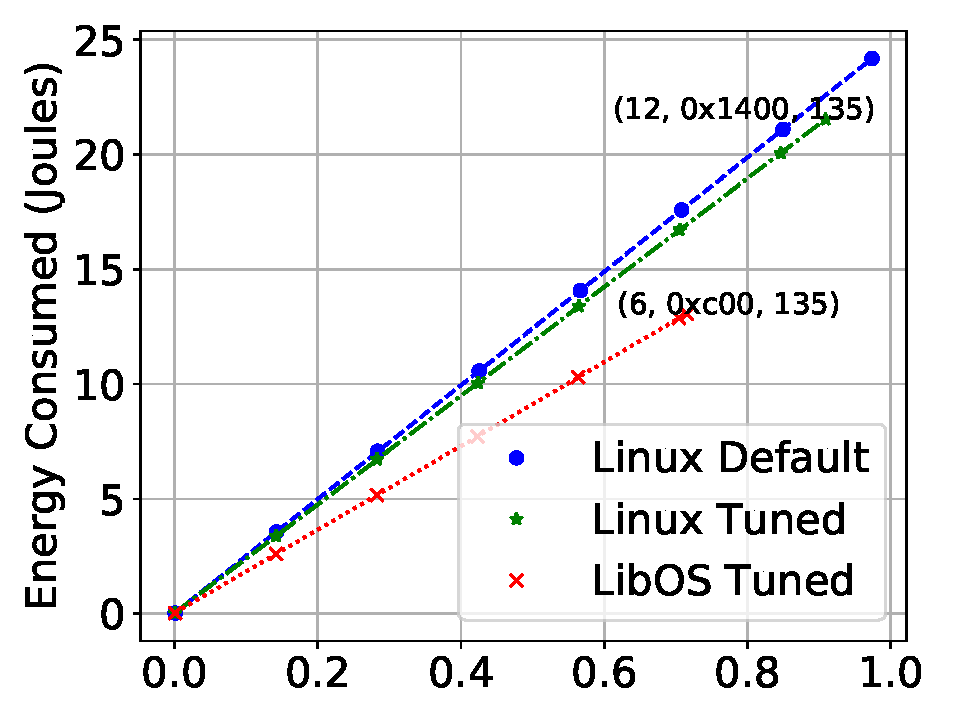
\includegraphics[width=\columnwidth]{osdi_figures/netpipe_65536_epp}
        \end{subfigure}
%        \hfill
        \begin{subfigure}[b]{0.35\textwidth}  
            \centering 
            \caption[]%
            {{Memcached:600K QPS}} 
            \vspace*{-0.25cm}    
            \label{fig:jl_mcd600}
            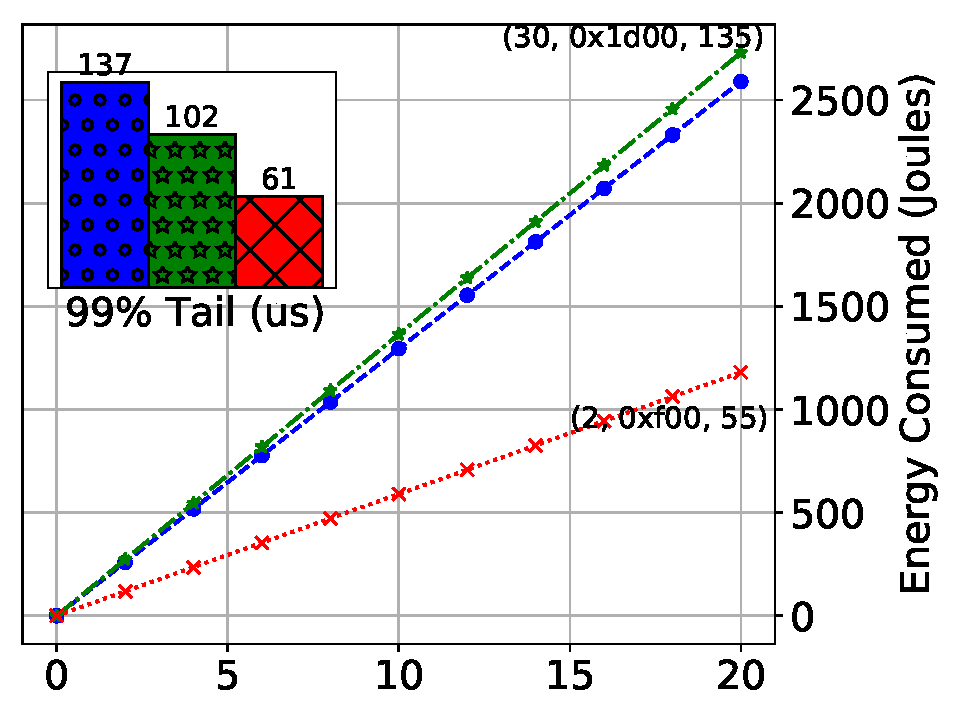
\includegraphics[width=\textwidth]{osdi_figures/mcd_600000_epp}
        \end{subfigure}
        \vskip\baselineskip
        \vspace*{-0.64cm} 
        \begin{subfigure}[b]{0.35\textwidth}   
            \centering 
            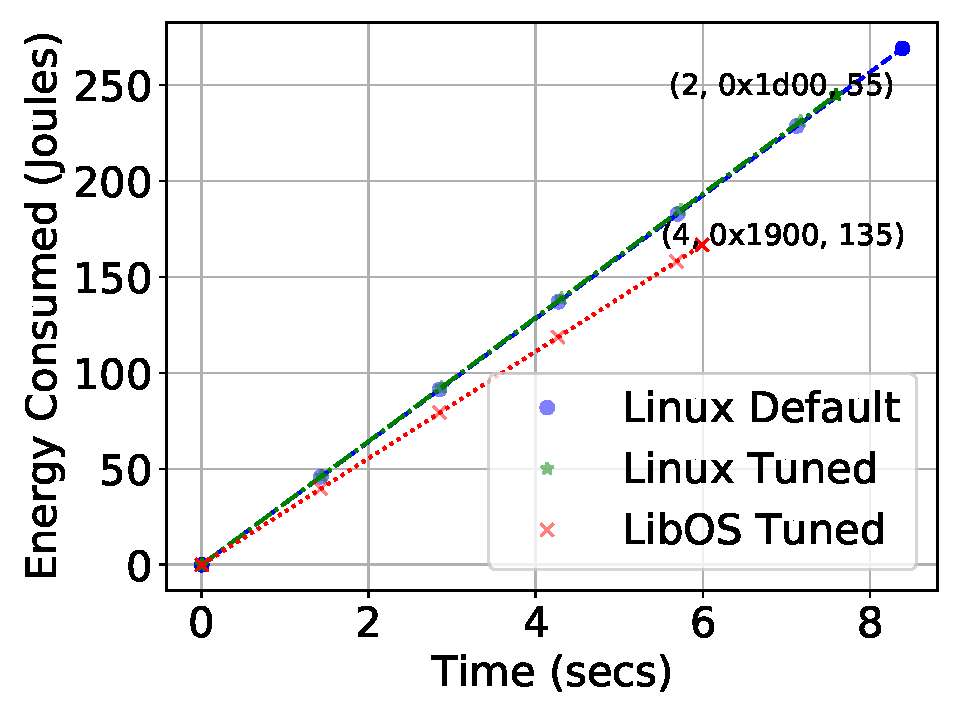
\includegraphics[width=\textwidth]{osdi_figures/nodejs_epp.pdf}
            \caption[]%
                    {{NodeJS}}
                    \vspace*{0.15cm}
            \label{fig:jl_nodejs}
        \end{subfigure}
%        \hfill
        \begin{subfigure}[b]{0.35\textwidth}   
            \centering 
            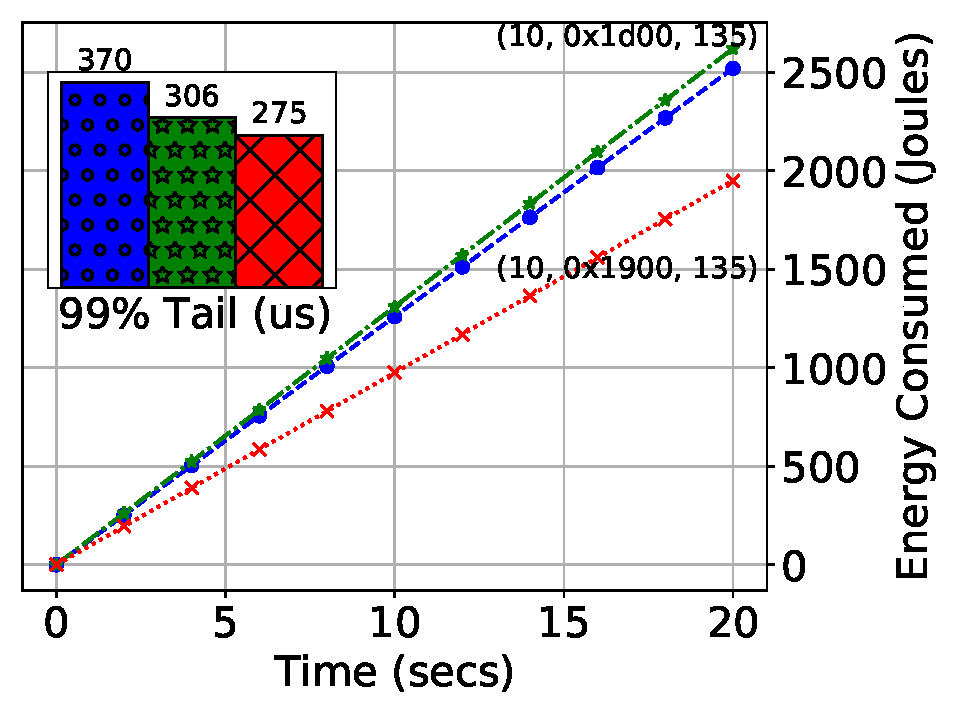
\includegraphics[width=\textwidth]{osdi_figures/mcdsilo_200000_epp}
            \caption[]%
            {{Memcached-silo:200K QPS}}
            \label{fig:jl_mcdsilo200}
        \end{subfigure}
        \caption[]
        {EPP timelines: For each workload we identify the unique hardware settings, for both Linux and libOS, that resulted in the systems best (min) Energy Performance Product (EPP) value. X-axis measures time for each workload (secs), both memcached's ran for 20 secs. The points on each line are a sub-sampling of energy use to improve legibility.
        %Using these values we plot a timeline of the joule readings for one experimental run at the setting for Linux tuned and libOS along with data from a default Linux run of the workload.  The x-axis is the time offset from the beginning of the experiment.  For each log entry with a joule reading, we plot its value against its timestamp offset from the beginning of the run.  While the log has entries for every interrupt, we restrict sampling the joule counter to be at least 1ms apart as per the hardware manual's recommendation, as such not all log entries have an associated joule value.  To improve readability we only show a subset of the markers and use a line to connect the visible marks to the points not shown.    
        } 
        \label{fig:epp}
    \end{figure*}

      \begin{figure*}
        \centering
        \begin{subfigure}[b]{0.35\textwidth}
            \centering
            \caption[]%
            {{Netpipe:64 KB Message}}  
            \vspace*{-0.25cm}  
            \label{fig:metrics_netpipe64}
            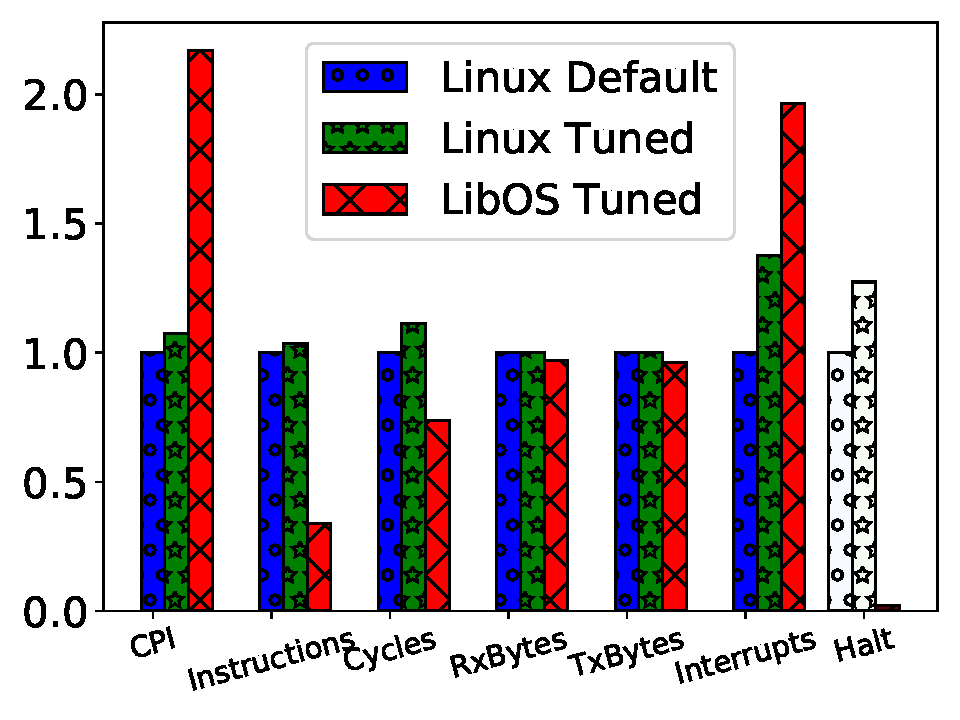
\includegraphics[width=\columnwidth]{osdi_figures/netpipe_65536_barplot}
        \end{subfigure}
 %       \hfill
        \begin{subfigure}[b]{0.35\textwidth}  
            \centering 
            \caption[]%
            {{Memcached:600K QPS}} 
            \vspace*{-0.3cm}    
            \label{fig:metrics_mcd600}
            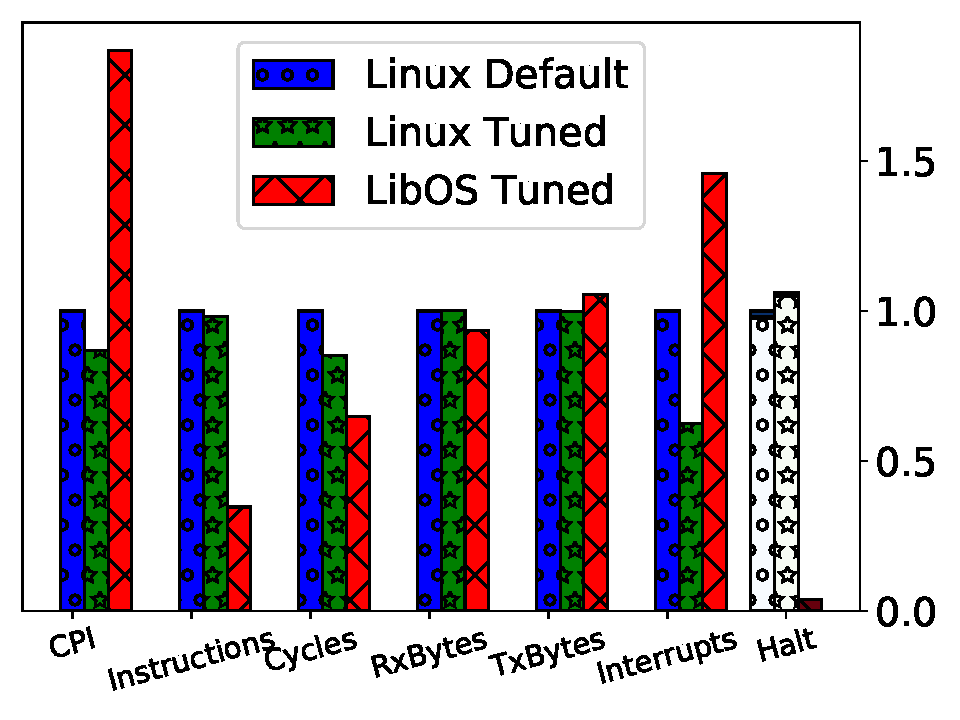
\includegraphics[width=\textwidth]{osdi_figures/mcd_600000_barplot}
        \end{subfigure}
        \vskip\baselineskip
        \vspace*{-0.4cm} 
        \begin{subfigure}[b]{0.35\textwidth}   
            \centering 
            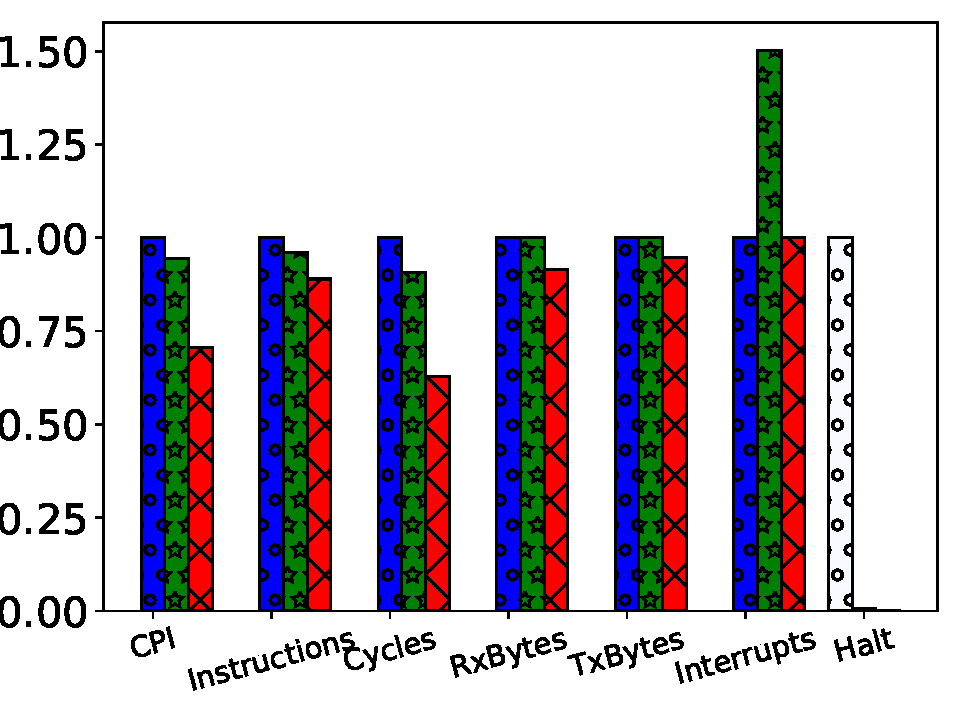
\includegraphics[width=\textwidth]{osdi_figures/nodejs_barplot.pdf}
            \caption[]%
            {{NodeJS}}    
            \label{fig:metrics_nodejs}
        \end{subfigure}
 %       \hfill
        \begin{subfigure}[b]{0.35\textwidth}   
            \centering 
            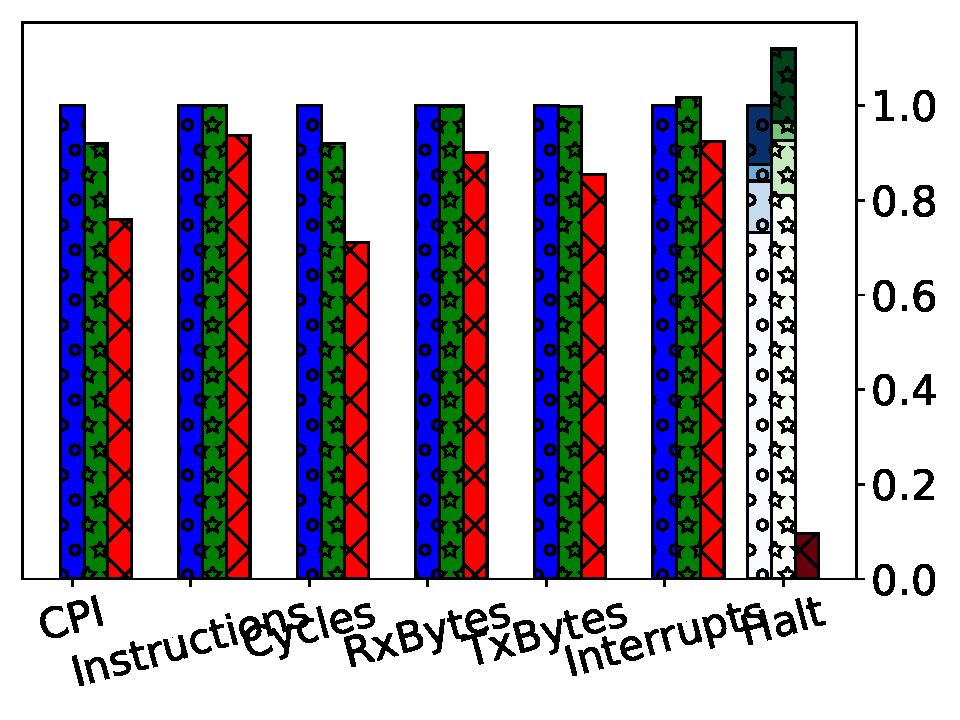
\includegraphics[width=\textwidth]{osdi_figures/mcdsilo_200000_barplot}
            \caption[]%
            {{Memcached-silo:200K QPS}}    
            \label{fig:metrics_mcdsilo200}
        \end{subfigure}
        \caption[]
        {Aggregate metrics from selected runs normalized against Linux default: For each experimental run, we instrument a detailed log entry collection in order to capture a set of hardware and software statistics. The halt bar shows the set of sleep state counts from C1 (lightest color) to C7 (darkest color) stacked on top of each other. %Each bar plot is a summation of all entries for that value in the per-interrupt log. 
        %Instructions and (unhalted) cycles are measured at a 1 ms timescale from reading Intel's PMC registers. Receive and transmitted bytes are read from the NIC's device driver data structures. The number of interrupts is measured as the length of all entries in a single experimental log. The halt bar shows the set of sleep state counts: [\texttt{C1}, \texttt{C1E}, \texttt{C3}, \texttt{C6}, \texttt{C7}], in Linux they are read from a the idle scheduler's data structure and in the libOS we keep a global counter before every \texttt{halt} instruction is called. 
        }  
        \label{fig:metrics}
    \end{figure*}%    

      \begin{figure*}
        \centering
        \begin{subfigure}[b]{0.35\textwidth}
            \centering
            \caption[]%
            {{Netpipe:64 KB Message}}  
            \vspace*{-0.25cm}  
            \label{fig:busy_netpipe64}
            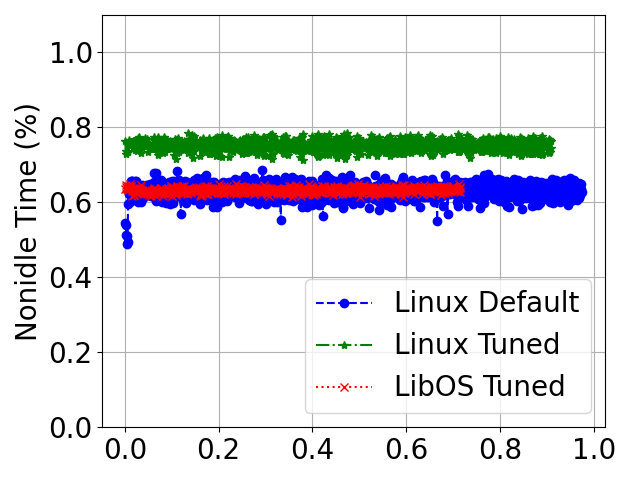
\includegraphics[width=\textwidth]{osdi_figures/netpipe_65536_nonidle_timeline.png}
        \end{subfigure}
        %\hfill
        \begin{subfigure}[b]{0.35\textwidth}  
            \centering 
            \caption[]%
            {{Memcached:600K QPS}} 
            \vspace*{-0.25cm}    
            \label{fig:busy_mcd600}
            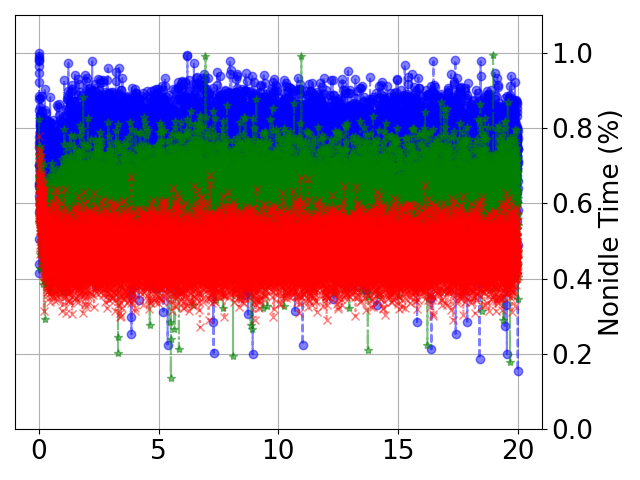
\includegraphics[width=\textwidth]{osdi_figures/mcd_600000_nonidle_timeline.png}
        \end{subfigure}
        \vskip\baselineskip
        \vspace*{-0.62cm} 
        \begin{subfigure}[b]{0.35\textwidth}   
            \centering 
            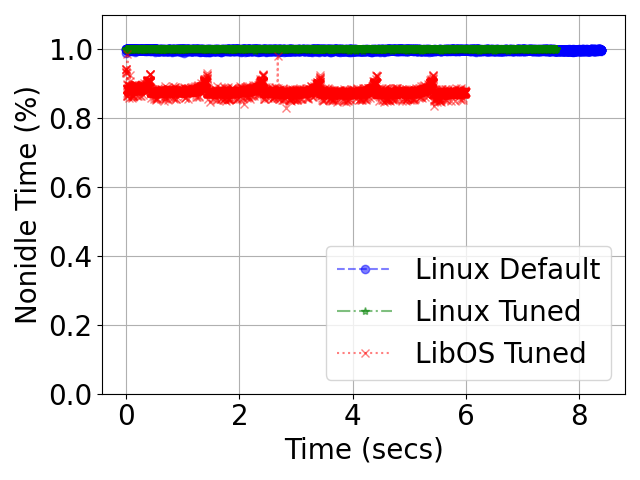
\includegraphics[width=\textwidth]{osdi_figures/nodejs_nonidle_timeline.png}
            \caption[]%
            {{NodeJS}}    
            \label{fig:busy_nodejs}
        \end{subfigure}
        %\hfill
        \begin{subfigure}[b]{0.35\textwidth}   
            \centering 
            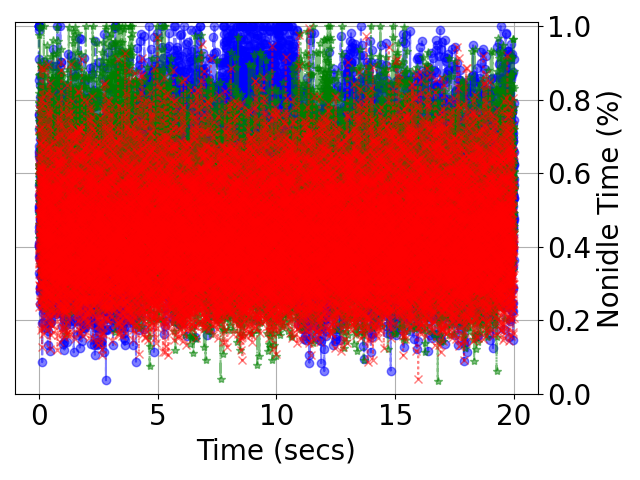
\includegraphics[width=\textwidth]{osdi_figures/mcdsilo_200000_nonidle_timeline.png}
            \caption[]%
            {{Memcached-silo:200K QPS}}    
            \label{fig:busy_mcdsilo200}
        \end{subfigure}
        \caption[]
        %% TODO
        {Busy timelines from selected runs:  Non-idle time is computed as the ratio between (un-halted) cycles and the time difference between every reading of timestamp register.}
        \label{fig:busy}
    \end{figure*}%    

      \begin{figure*}
        \centering
        \begin{subfigure}[b]{0.35\textwidth}
            \centering
            \caption[]%
            {{Netpipe:64 KB Message}}  
            \vspace*{-0.25cm}  
            \label{fig:joule_netpipe64}
            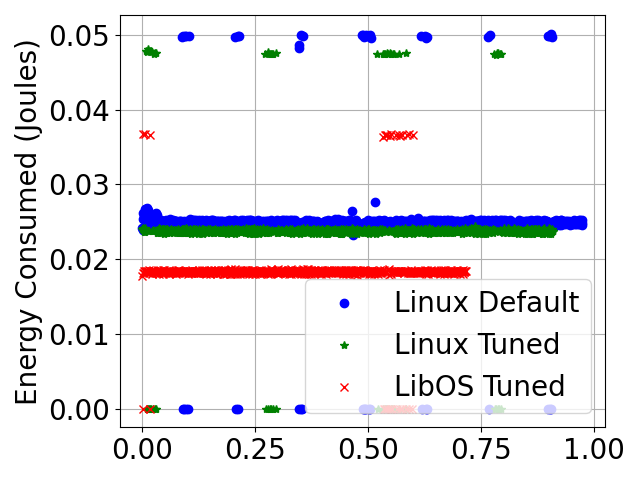
\includegraphics[width=\textwidth]{osdi_figures/netpipe_65536_joule_timeline.png}
        \end{subfigure}
     %   \hfill
        \begin{subfigure}[b]{0.35\textwidth}  
            \centering 
            \caption[]%
            {{Memcached:600K QPS}} 
            \vspace*{-0.25cm}    
            \label{fig:joule_mcd600}
            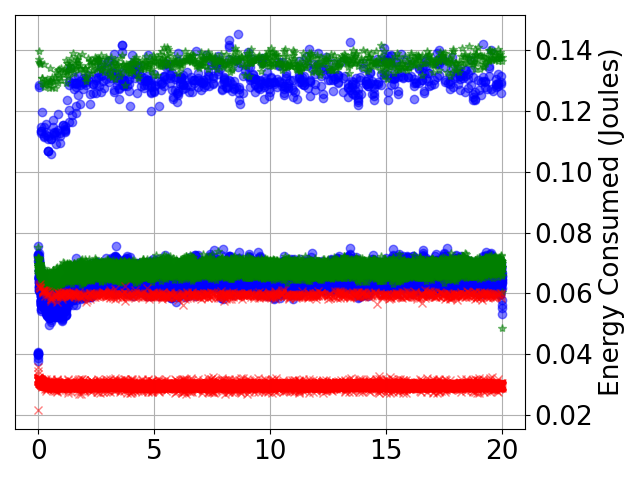
\includegraphics[width=\textwidth]{osdi_figures/mcd_600000_joules_timeline.png}
        \end{subfigure}
        \vskip\baselineskip
        \vspace*{-0.62cm} 
        \begin{subfigure}[b]{0.35\textwidth}   
            \centering 
            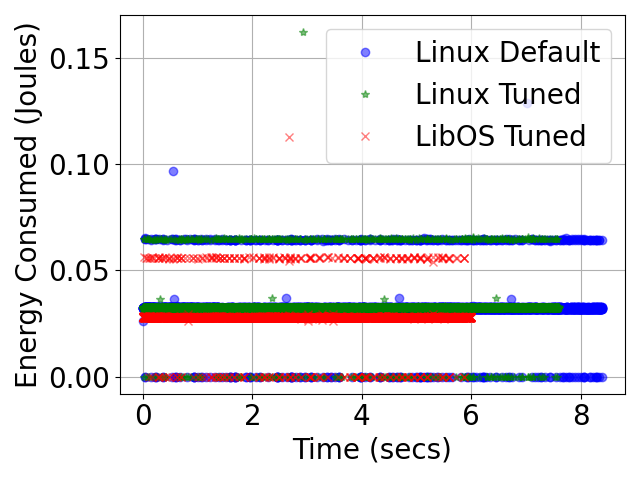
\includegraphics[width=\textwidth]{osdi_figures/nodejs_joule_timeline.png}
            \caption[]%
            {{NodeJS}}    
            \label{fig:joule_nodejs}
        \end{subfigure}
       % \hfill
        \begin{subfigure}[b]{0.35\textwidth}   
            \centering 
            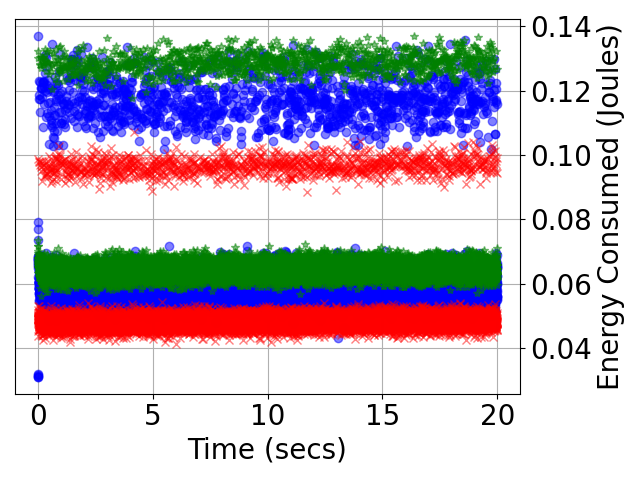
\includegraphics[width=\textwidth]{osdi_figures/mcdsilo_200000_joules_timeline.png}
            \caption[]%
            {{Memcached-silo:200K QPS}}    
            \label{fig:joule_mcdsilo200}
        \end{subfigure}
        \caption[]
        {Energy timelines from selected runs:  Joule difference between every 1 ms reading of joule register plotted against time of entire experimental run.} 
        \label{fig:joule}
    \end{figure*}%  


\section{Observations}

In this section,
we present observations from our curated study.
We begin with a discussion of broad overview observations.
This overview utilizes four landscape plots (see Figures ~\ref{fig:netpipe64Kov} -~\ref{fig:mcdsiloov}) that each summarize thousands of related  experiments.
We then move on to detailed observations that use log data from each workload
to construct interesting analysis points.
To ease comprehension, we have included the bulk of data plots we refer to.  
%Each figure is composed of four subplots arranged in a manner to make cross workload analysis easier.
This section will often refer back to the questions posed in the introduction
as our observations shed light on them.

\subsection{Overview}
\label{sec:resoverview}
%%
% summary landscape plots
%
      \begin{figure*}[t]
        \centering
        \begin{subfigure}[b]{0.45\textwidth}
            \centering
            \caption[]%
            {{\small Netpipe 64 KB message}}  
            \vspace*{-0.3cm}
            %\hspace*{0.35cm}  
            \label{fig:netpipe64Kov}
            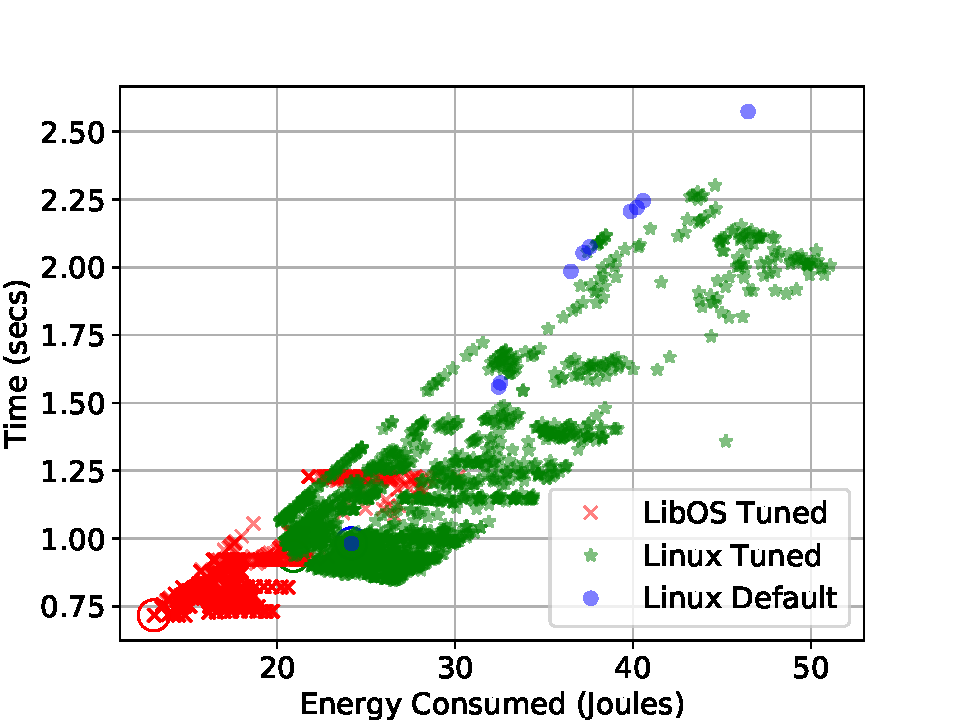
\includegraphics[width=\textwidth]{osdi_figures/netpipe_65536_overview.pdf}
        \end{subfigure}
%        \hfill
        \begin{subfigure}[b]{0.45\textwidth}  
            \centering 
            \caption[]%
            {{\small Memcached 600K QPS}} 
            \vspace*{-0.25cm}    
            \label{fig:mcdov}
            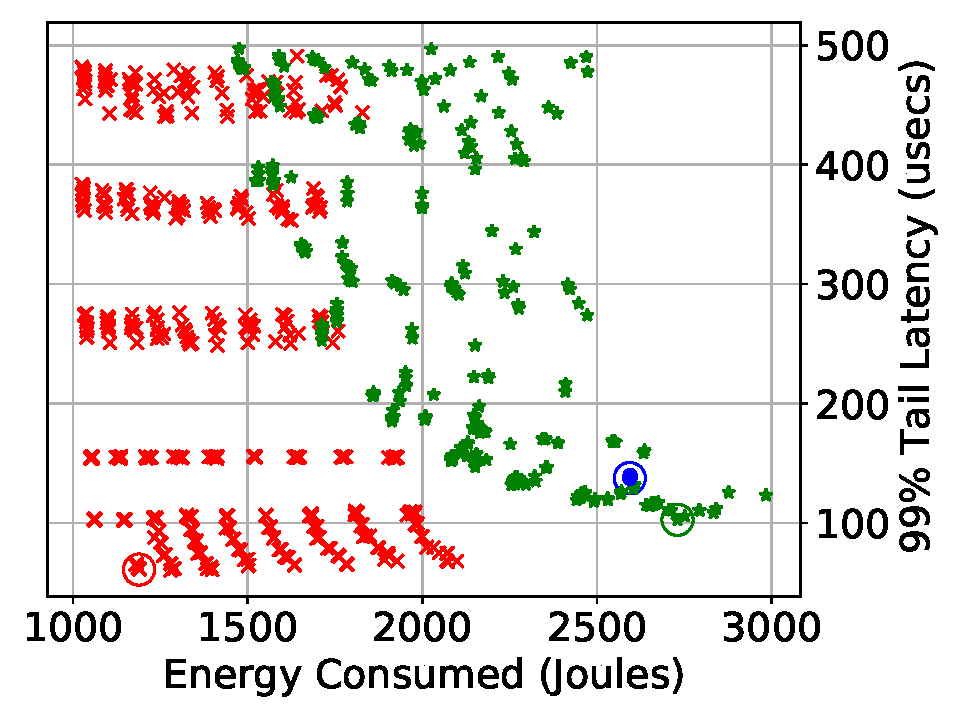
\includegraphics[width=\textwidth]{osdi_figures/mcd_600000_overview.pdf}
        \end{subfigure}
        \vskip\baselineskip
        \vspace*{-0.47cm} 
        \begin{subfigure}[b]{0.45\textwidth}   
            \centering 
            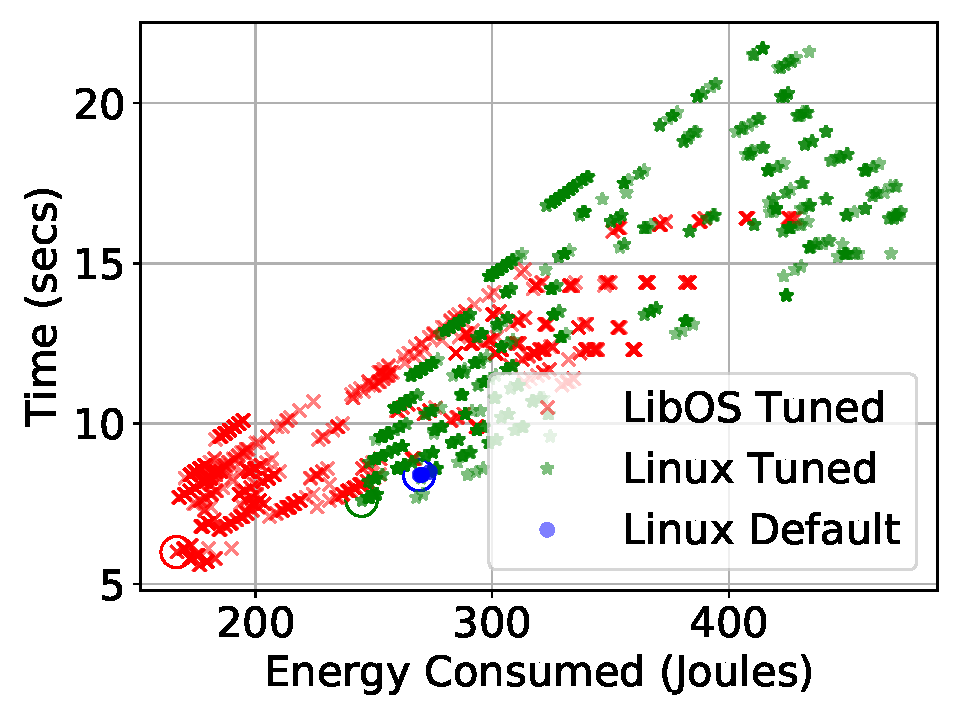
\includegraphics[width=\textwidth]{osdi_figures/nodejs_overview.pdf}
            \caption[]%
                    {{\small NodeJS 100K requests}}
                    %\hspace*{0.35cm}  
            \label{fig:nodejsov}
        \end{subfigure}
%        \hfill
        \begin{subfigure}[b]{0.45\textwidth}   
            \centering 
            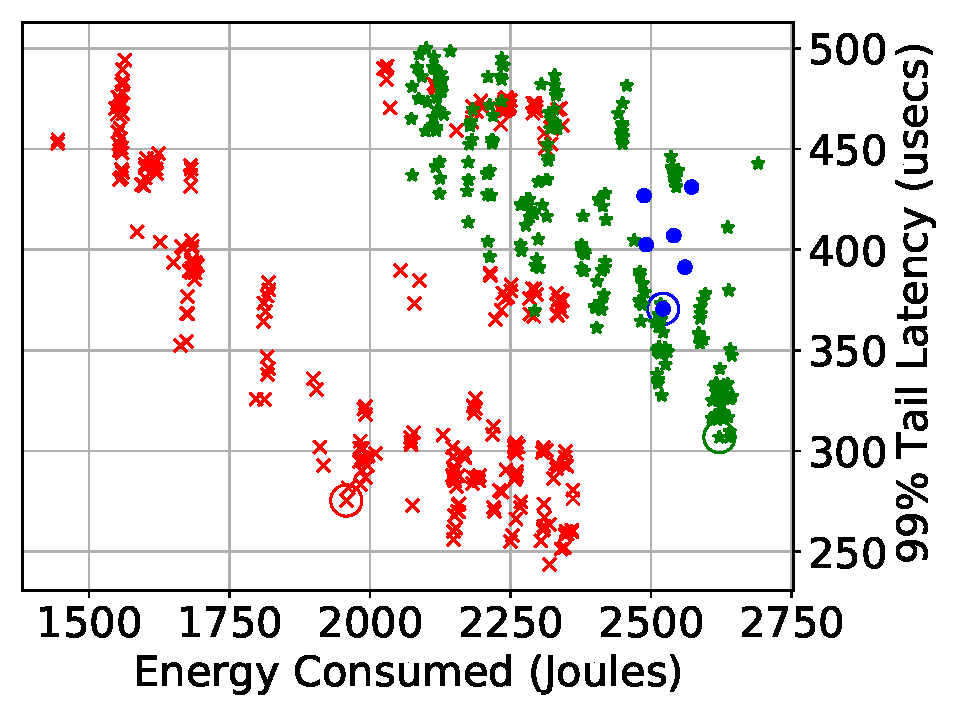
\includegraphics[width=\textwidth]{osdi_figures/mcdsilo_200000_overview.pdf}
            \caption[]%
            {{\small Memcached-silo 200K QPS}}    
            \label{fig:mcdsiloov}
        \end{subfigure}
        \caption[]
                {\small
These landscape plots portray the space of energy-performance profiles
that an OS/workload software stack can exhibit. The circle around individual points represent the min EPP values achieved in each workload.
\textit{Note that, in these plots, the origins do not start at zero
because the aim of the plots is to highlight structure within a plot
rather than to draw a comparison across plots.}
                  %Data from a run the settings associated with the 'best' EPP points are presented in~\ref{sec:data} and discussed in~\ref{sec:details}.          %Using these values we plot a timeline of the joule readings for one experimental run at the setting for Linux tuned and libOS along with data from a default Linux run of the workload.  The x-axis is the time offset from the beginning of the experiment.  For each log entry with a joule reading, we plot its value against its timestamp offset from the beginning of the run.  While the log has entries for every interrupt, we restrict sampling the joule counter to be at least 1ms apart as per the hardware manual's recommendation, as such not all log entries have an associated joule value.  To improve readability we only show a subset of the markers and use a line to connect the visible marks to the points not shown.    
        } 
        \label{fig:overview}
    \end{figure*}



Figure~\ref{fig:overview} illustrates energy-performance landscapes that summarize all the experiments for four of the eleven workloads runs (~\ref{table:wrkcfgs}).  Each point in these graphs represents a single experimental run.  Using log data for a run, we calculate the total energy consumed along with a workload-specific performance measure. For both memcached and memcached-silo, we filter any results that do not satisfy an SLA of 500 $\micro s$. In the performance metrics of both closed loop and open loop workloads, better in both cases is indicated by a lower value. Therefore, the best performance and energy states form a pareto-optimal energy-performance curve of points that are closest to the origin in the landscape plots.  

%In netpipe and nodejs, the workload-specific measure we use is the time taken to complete a fixed number of sequential transactions in a closed-loop setting.  For netpipe (figure~\ref{fig:netpipe64Kov}), we measure the time taken to complete 5000 round-trips between a client and server configured with the same OS and hardware settings for a fixed message size of 64 KB.  For nodejs (figure ~\ref{fig:nodejsov}), we measure the time required to serve 100,000 HTTP requests.

%In the open-loop workloads, memcached and memcached-silo, the performance metric used is the 99\% tail latency specific queries-per-second (QPS) load sustained for a period of 20 seconds.
%In memcached (figure~\ref{fig:mcdov}), we apply an offered load of 600K QPS generated using the ETC Facebook benchmark~\cite{mutilate}.
%For memcached-silo (figure~\ref{fig:mcdsiloov}), we apply a load of 200K QPS. Note that, in both open-loop cases, the offered loads are close-to but do not exceed the maximum system's capacity (~\ref{sec:perf_baseline}).  
%Furthermore, for both memcached and memcached-silo, we filter any results that do not satisfy an SLA of 500 $\micro s$.  
%Each experimental run uses a unique setting for the three hardware settings we study (ITR, DVFS, and RAPL).

%Given that we use total time for a fixed amount of work in the close loop settings and we use 99\% tail latency in the open loop settings as performance metrics, better in all cases is indicated by a lower value. The relative value of one point versus another in figure~\ref{fig:overview} depends on what value/utility one places on the importance/cost of energy versus performance.


To enable analysis we will use the product of Energy and Performance  (EPP), as a single quantity ($Joules \times Performance$) to rank points. EPP is one simple way of comparing individual results as points with lower EPP represent a systems ability to achieve an overall better result in the tradeoff space. Figure~\ref{fig:overview} also include circles drawn around the points with the overall min EPP achieved for the each OS configuration studied. Across all the workloads, tuning libOS was able to achieve up to 74\% EPP savings over Linux. In section~\ref{sec:q1_2} we will examine how differences in OS path length and efficiency plays a role in these results. We also find that tuning Linux could achieve EPP savings up to 48\% over its default behavior. This demonstrates, independent of OS design and implementation changes a general purpose OS can do better on a dedicated workload with a simpler static policy.

%The landscape plots suggests that the OS has a fundamental influence on the energy-performance profile that can be achieved over the range of the three hardware settings swept.  Running a dedicated application with a libOS structure results in significant pareto-optimal energy-performance benefits. In all the landscapes plots, including those not shown, the library OS has a pareto-optimal curve that is closet than that of the Linux.  The gap is unsurprinsgly less pronounced for the open loop workloads at the lowest load. 

The landscape plots also reveal that the OS response to the various settings has two interesting phenomena.  First, both OS' have a relatively clear pareto-optimal curve that identifies the setting for which there exists energy performance tradeoffs that an administrator might want to exploit. A system with only one point at a lower EPP may not be as useful as a system that has many distinct points at similar EPPs; such points allow tuning for one's utility and cost or adjust to changes in utility and costs. Second, we can see more distinct structure within the libOS in the open loop workloads~\ref{fig:mcdov}~\ref{fig:mcdsiloov}, we find these small bands are placed by their respective ITR-delay values and the small points within each band is a search through DVFS and RAPL space. We attribute the simplicity of the libOS to demonstrating this structure, which argues policies built in the libOS can be simpler and more effective.
%Second, someone hoping to tune manually or in an automated fashion should be aware that many settings do not fall on the parateo-optimal curve and care must be taken to avoid choosing bad settings.
 
%functionality of the OS plays by examining the more detailed data.  

%When only considering EPP we found across the sweep of the three hardware parameters across all the workloads the best EPP achieved by the library OS was from X to Y better than the best EPP achieved with Linux.  

%Focusing on the Tuned Linux points in comparison to the default Linux behaviour



%Linux's default behaviour is closest to the optimal behaviour achieved with a static tuning in Memcached.  On the other workloads as visible in the landscapes the default behaviour can suffer high variability, which swings its realized energy or time quite far from optimal, or even if stable its mean can still be suboptimal.  To see this consider figure~\ref{fig:mcdov}.  While the default points are tightly clustered if the same tail latency could be achieved via manual tuning for approximately 400 less Joules over the 20 second period (using the horizontal intercept of the default cluster at P,Q the furthest left Tuned Linux point M,N represents equivalent tail latency at an energy consumption of M).

%More generally comparing best case mean EPPs we observed, across all workloads that statically tuning Linux results in X-Y\% lower EPP compared to how its default behaviour.  

% to do not sure this belongs here on in the discussion. 
%The above observation suggests that the complex OS energy management, design and implementation, do not easily result in optimal behaviour for a fixed workload.  While static tuning can improve the behaviour it is hard to tell how much better the results could be if dynamic energy management were more systemically removed or turned off.  In some sense the library OS does represent such a contrast but it of course is a more radical departure.  

  
 %todo it would be nice to quantify EPP ranges and how many diverse settings have equivalent EPPs as this is also very cool to know... can't be told from the landscapes as we can't see the settings... this is really a more detailed finding but global in a data sense. 

%Discuss any other overview details here that don't easily fit in the analysis section.





\subsection{Results and Analysis}
\label{sec:analysis}


%\subsubsection{Does length matter?}

\paragraph{Length matters(Q1):} Perhaps unsurprisingly, the use of a library OS, designed and implemented to run a single dedicated application, results a dramatic reduction (50-75\%) in the number of instructions required in the two OS dominate workloads, Netpipe and Memcached across all packet sizes, when configured for the best EPP (minimum time and energy).   
To better understand this effect we focus on the Memcached results and utilize the detailed data from one run of Linux and the libOS when then achieve their best EPP (subplots 3b, 4b, 5b and 6b).   

Figure 3b, a plot of the energy time line of a best EPP run for both Linux tuned and the libOS and a Linux default, clearly shows that here is a clear reduction in both tail latency (56\% of Linux Tuned) and the energy consumed (40\% of Linux Tuned).  This translates to a 74\% EPP reduction. The plot also shows that the rate of energy consumption is lower in the library OS. 

%todo: this paragraph can go
Examining the aggregate metrics plot 4a corroborates that indeed there is a dramatic (65\% reduction) difference in the number of instructions used to complete the work. 
Unsurprisingly when statically setting Linux to the values we found to produce the optimal behavior there is not substantial  difference in the number of instructions that Linux requires to do the work.

\vspace{-.2in}
\paragraph{OS Adaptation (Q3):} 
What is surprising is that while the Library OS has a reduced instruction length its instruction efficiency (Cycles Per Instruction, CPI) is actually worse at its best EPP. 
So, while it saved 65\% in instructions, it actually only saves 24\% of the time executing instructions.  
This indicates that there is another effect that is resulting the the large EPP savings we see. 
%If this was the only savings then we would not expect the as large a saving in EPP we see.  

%The impact of the reduced path length induces a fascinating effect.
When we examine  the time between interrupts, we see that the mean non-idle time is approximately 24\% lower than that of Linux tuned.  
However, while the systems handle approximately the same number of interrupts, the number of times the library OS halts is dramatically lower than that of Linux.    
Our expectation was that the explanation would come from the difference in idle behavior between the operating systems
%At first glance one suspects that the clear explanation must come from a difference in idle behavior.  

While true, it turns out that it was not in the way we expected.  
Examining 6a, a time line plot of the energy consumed on a representative core between (1 ms separated) interrupts, we see two interesting facts.  
First, across systems a core seems to, as expected, switch between two energy states, high  and low -- busy and idle respectively.  
Second, the library OS's best EPP emerges in such a way that the energy it consumes when busy is actually lower than the energy of Linux Tuned consumes when idle and on the lower end of Linux default.  

One would assume reducing the number of instructions  would naturally open up idle time to be spent in a halted state.  
But given the interplay between the various constants associated with the processor sleep states and the saving had from slowing the processor down it actually pays to not use a configuration that results in a race-to-halt strategy.  
Rather given the library OS simple idle behavior (halt to C7) best EPP results from slowing the processor down and reducing the cost of busy consumption despite it lengthening the busy time which of course comes at the cost of not halting.  

\vspace{-.2in}
\paragraph{Impact of Complexity (Q4):} Fundamentally, it is the headroom in the number of required instructions to do the work that allows this response to adjusting the RAPL and DVFS settings.
Linux on the other hand despite having complex halt algorithms settles on its best EPP when the processor is run at its maximum power setting during the busy time, in contrast to the library OS which runs the processor in its lowest setting during busy intervals.
Thus Linux races to halt, halting many more times, for a shorter period but with at a lower sleep state. 

Overall, we see is that the reduced path length of the libOS has both a direct result ({\bf Q1}) on energy, and provides the libOS the opportunity to slowdown, exploiting an unexpected  ({\bf Q3}) strategy that achieves better performance and energy. 
We hypothesize that Linux does not seem to be able exploit this same strategy, in part because its path lengths are too long, and in part because its sophisticated energy halt behavior ({\bf Q4}) that constantly changing halt state, while in a small time scale having strong advantages over the simple libOS policy, interfere with it adopting a steady state globally more optimal performance.  


\vspace{-.2in}
\paragraph{Impact on Applications (Q2):}
While it is interesting to see the effects of reducing the code path lengths, and how this interacts with energy consumption, is there any real impact from the OS design or implementation choices we make on application efficiency.  To probe this we examine the application centric workload, NodeJS and Silo-TPCc.  

Across these workloads our sweep of ITR, DVFS and RAPL reveals that the OS has significant impacts despite the application centric nature.  
When configured for best EPP we find that the library OS results in a 30\% and 25\% reduction in Joules and time respectively. Which translates to a 48\% EPP improvement.    
For Silo-TPCc, again configured for best EPP, we observe at the highest load we evaluate (600 KQPS) a 19\% and 20\% saving in energy and tail latency.  
In terms of EPP this is 35\% reduction.  
As we reduce load the EPP savings drops to 14\% and 1\% for 100 KQPS and 40 KQPS.  

Surprisingly, the OS must be having an impact on the busy component despite the busy time being dominated by the application.  
After all, NodeJS is closed loop and as such its inter-arrival will decrease as you increase performance and in the case of Silo-TPCc we see the improvements in EPP go up as a function of load.  

Again we will use details from one of the experimental runs to explore this effect.  
This time we will use the closed-loop workload of NodeJS to provide a contrast in our analysis (Figures 3c, 4c, 5c and 6c).  

In figure 3c, given that the time to completion is our performance metric the energy timeline reveals directly the EPP achieved at this setting. 
As such we can see the how the systems compare in both the energy and performance domain as the experiment runs.  
The reduction in slope between the Library OS and Linux tuned demonstrates that at the settings for best EPP (denoted by the labels at the the final point of each run) a lower rate of energy consumption.  

Unlike Memcached, we do not see a complete inversion in the hardware energy settings.  
Best EPP for Linux is achieved when the processor is at its highest values and for the library OS, while it is not the highest, it is a medium s6 DFVS setting (6 highest out of the possible 17). 
As we proceed we explore a fascinating behavior that arises as one sweeps energy setting on the Library OS.

Unlike the OS centric workloads the application centric, as expected, do not display a particularly discrepancy in the number of instructions required to accomplish the requisite work as illustrated in the metrics plots (4c and 4d).  
Surprisingly, however, we see an inversion in how CPI compares in the application centric workload versus the OS centric, across the two Operating Systems.  
Despite the fact that the instructions are application dominated CPI is actually improved in the Library OS despite the fact that the best EPP is being realized at a lower energy setting than Linux.  
Whereas the setting for Linux that achieves best EPP is running the processor at its highest setting to achieve the best performance and energy.

Close loop scenarios, with a fixed amount of work to accomplish, like  our NodeJS and Netpipe workloads, create a scenario which optimizing for time and energy can be roughly equivalent.  
Speeding up the work minimizes the time to receive your next packet upto the limit of transmission and processing needs on the other side.  In the case of NodeJS the transmission time is negligible and the other side's processing cost is also small.   


The library OS's structure results in an interesting modulation between two behaviors ({\bf Q3}).  
When we examine the number of interrupts that this workload induces across the operating systems as we vary the settings (this data has been removed in the interest of space).  
Linux largely executes 200K interrupts for all but the lowest settings of ITR at which point it suffers 300K interrupts.  
Examining our detailed timelines from several runs we see that the NIC asserts and interrupt for every received packet and a send acknoledge interrupt.  
However at the low ITRs the card fires a spurious interrupt such that every request introduces 3 interrupts. 

In the case of libOS when we examine the number of interrupts that occur we find a fascinating behavior.  
Despite this being a closed loop the OS is able to at different energy settings change its behavior ({\bf Q3}) between polling and interrupt driven IO.  

Given the nature of the execution model the event that handles an inbound request synchronously executes the application logic in NodeJS.  
This logic, imitates the send, which the device driver synchronously initiates, and then the application logic continues the expensive completion of the interpreted NodeJS logic.
Given the minimal transmission and processing time, when the application code completes, it returns back to the device logic, whose internal poll loop discovers a new packet available.  
This specific behavior arises when we slow the processor down just to the right speed.  
This is another expected emergent adaptation of the operating system ({\bf Q3}) to optimize energy and performance. 

% net cycles savings is 35% but our time and energy savings are 

% save more energy than time 
% best perf cpi: 
%           halts:
% best epp  cpi:    
%           halts:




%\subsection{Open Loop}
\label{sec:q2}
\begin{itemize}
\item Q3: How do different OSes exploit idle periods to halt and save energy?
\item Q4: How do different tuning impact different OSes?
\end{itemize}

%For open loop applications, if SLA is the most important (e.g., 99\% tail latency less than 500 \micro s) then the configuration with lowest absolute energy should always be selected. However, it may also be useful to consider a lower tail latency if it doesn't involve a dramatic increase in energy use. For both workloads, we find that Linux typically trades off increases in energy and decrease in tail latency to arrive at its min EPP setting while the libOS decreases both energy and tail latency.

Across the different QPSes in memcached, tuning Linux (30, 0x1d00, 135) can lower its EPP by up to 22\% while tuning the libOS (2, 0xf00, 55) can lower its EPP by up to 74\%. The libOS was able to set ITR, DVFS and RAPL all at lowest setting in memcached. This result is not surprsing given the throughput performances in ~\ref{sec:perf_baseline}, as a QPS of 600K is considered relatively light for the libOS while for Linux it is approaching its peak. Examining the log data we also find that in the min EPP across all the QPS loads, tuned Linux typically increased of its energy by 5\%-10\%  and reduced its 99\% tail latency by 18\%-26\%, whereas libOS' was able to reduce both energy and tail latency by up to 40\% and 56\% respectively. For memcached-silo, we see similar trade-offs of energy (4\%-7\%) for lower tail latency (22\% - 37\%) in Linux tuned and both a reduction in energy (39\%-48\%) and tail latency (24\%-38\%) in libOS. Given the processing heavier aspects of memcached-silo the DVFS and RAPL values are all set at higher values. However, we still see the libOS being able to lower its DVFS and RAPL to lower levels compared to Linux tuned. The ITR delay has also increased in both libOS and Linux to a range between 10 \micro s-40 \micro s.

%For the libOS, we find in all the three QPS loads, the best ITR value was 2 \micro s; which is the lowest value examined. For tuned Linux, the best ITR values range from 10 \micro s at 200k QPS up to 30 \micro s at 600K QPS. At 200K and 400K QPS, tuned Linux set its DVFS and RAPL at the median ranges and at the highest QPS load of 600K, Linux tuned set DVFS and RAPL at the highest value. 

%In memcached for 200K,400K QPS, Linux tuned had higher number of interrupts than defaults, likewise had higher number of halt states called than Linux default, however the number of energy use increased - a low static ITR at low QPS causes work to be done fast, wakes up idle scheduler and and causes more sleep states to be used, however this could indicate the algorithm isn’t performing as efficiently as even though number of sleep states used increased, the energy used increased as well, indicating the time to sleep actually was much shorter and therefore incur extra costs.

Another interesting tradeoff can be observed in overview figure~\ref{fig:mcdov}, where tuned Linux can drastically lower its energy consumption by up to 50\% if it is willing to sacrifice most of its 500 \micro s SLA budget. We find this is possible by aggressively setting ITR delay at much higher values of 300-400 \micro s. Using an 600K QPS in memcached as an example, we find that compared to default Linux, a tuned Linux with an ITR delay of 300 \micro s can lower its energy use by 44\% through a combination of: 1) 93\% reduction in total interrupts, 2) 30\% reduction in instruction use and last-level cache misses, and 3) a 12X increase in C1E, C3 sleep states, and 2X increase in C7 sleep states. To summarize, tuning Linux with a high ITR delay allows it to go to deeper sleep states and more often, further, the amount of reduced interrupt contents also contributed to less code being executed overall. Moreover, we find that it is able to lower its DVFS at a lower level than tuned Linux for minimum EPP, we hypothesize this is related to the fewer amount of non-application related work that is being done. We do not observe this dramatic of an energy savings in the libOS (only 14\% at 600K QPS), we suspect this effect comes into play at greater efficiences only at much higher QPS for the libOS. There have been a plethora of past work in reducing energy use of workloads such as memcached as it exhibits a diurnal pattern where periods of low utilization exist~\cite{hotpower2008, powernap, napsac}, tuning ITR delay can be an additional lever to further reduce a systems' overall energy use. We also find this trade-off to exist in memcached-silo where in tuned Linux can save energy by up to 47\%, and for the libOS, a smaller fraction of additional energy savings of up to 14\% can be gained.



%\subsection{Application Light}
\label{sec:q3}
\begin{itemize}
\item Q1: Impact of OS paths?
\item Q4: How do different tuning impact different OSes?
\end{itemize}

% What if any impact does OS path length and hardware tuning have on energy consumption?
%Application specific libOS' written for datacenter workloads often focuses on optimizing packet processing path lengths~\cite{ix, arrakis, ebbrt, farm}. Netpipe and memcached are two examples where the majority of processing is in the OS packet receive paths, given that the application compute portion is simpler in both. Examining the differend offered loads in both workloads, we find that: 1) across all four message size in netpipe, libOS used 6\%-77\% fewer instructions than Linux, and lowered its EPP by 37\%-80\%, and 2) across all three QPS in memcached, libOS used 71\%-75\% fewer instructions than Linux, and lowered its EPP by 41\%-74\%. 

Shorter path length in libOS allows it to expose gaps in packet inter-arrival rates in order to save more energy by further reducing its processor frequency and take advantage of halting. In netpipe 64 KB, figure~\ref{fig:metrics_netpipe64} shows libOS uses 67\% fewer instructions than Linux,  even though figure~\ref{fig:jl_netpipe64} shows that the libOS is able to use a lower ITR delay of 6 \micro s versus tuned Linux's of 12 \micro s, libOS is actually still less busy than Linux tuned (figure~\ref{fig:busy_netpipe64}). This instruction efficiency allows libOS to set DVFS at a lower frequency of 0xc00 versus tuned Linux's of 0x1400 to further reduce its energy consumption. In contrast to libOS, tuning Linux mainly uses similar amount of instructions as default or more instructions. Figure~\ref{fig:metrics_netpipe64} shows tuning Linux uses 17\% more instructions while having a lower EPP by 16\% as compared to default. This is partly due to the 40\% increase in interrupts for Linux, which adds additional interrupt handling instruction overhead. While these additional instructions and interrupts cause Linux tuned to be more busy (figure~\ref{fig:busy_netpipe64}), the data in figure~\ref{fig:joule_netpipe64} indicate tuning Linux consumed less energy. We hypothesize this could be an effect of the ITR delay value affecting Linux's scheduler such that tuned Linux was able to call halt instruction 39\% more than Linux default.

Given that memcached is a less compute intensive workload, it is not a surprise that reducing tail latency is more important for both tuned Linux and libOS. However, what is surprising is the different combination of ITR, DVFS, and RAPL settings that each system took. The libOS used the lowest ITR value possible (2 \micro s) and set its DVFS/RAPL at the median ranges, and while this resulted in a 50\% increase in number of interrupts compared to Linux default, the general efficiency and smaller size of the libOS can be seen in figure~\ref{fig:metrics_mcd600} as even with the extra interrupt counts, the libOS' instruction count was 65\% less than Linux. This efficiency enables libOS to minimize its 99\% tail latency while using less energy. Even though figure~\ref{fig:metrics_mcd600} also shows that the libOS went to C7 sleep state over 2X more than Linux default, we do not believe it actually stayed in those a C7 sleep state given its exit latency (hundreds of \micro s) and the dynamic nature of the workload with such a low ITR delay that will constantly wake up the processor. The biggest indication of tuned Linux's difference from default Linux is in the interrupt count, which is 30\% less than Linux default, we attribute this to its ITR delay value of 30 \micro s. This ITR delay seems to shift the ratio of sleep states to focus on C1 and C1E, overall it seems tuning Linux allows it to halt more often than Linux default. Figure~\ref{fig:metrics_mcd600} supports this by showing that tuning Linux spent less time being busy than default.

%Tuned linux has lower CPI than default, an indication of why it managed to achieve lower tail latency. While tuned Linux was able to be scheduled to sleep more often, it consumed energy at a higher rate than default, could be the exit latencies of more sleep states given the dynamic nature of memcached workload.

%

%\subsection{Application Heavy}
\label{sec:q4}
\begin{itemize}
\item Q2: Impact of OS in application heavy
\item Q4: How do different tuning impact different OSes?
\end{itemize}

In figures~\ref{fig:metrics_netpipe64}-~\ref{fig:metrics_mcdsilo200}, one can see at the CPU light workloads that while the libOS used drastically fewer instructions than Linux by up to 70\%, its CPI was actually up to 2X worse. This increase in CPI may be explained by the fact that libOS currently only goes into the deepest level of sleep (C7) while the majority of sleep states for linux are at lower level. In both workloads, the libOS' min EPP setting used a fast ITR delay of 2 \micro s, having such frequent interrupts to wake up the core means a C7 sleep state may not be the most optimal decision. It is also possible that the libOS is executing less wasted instructions that tend to be executed with a low CPI. Interestingly, we find changing OS' has an impact on application level CPI, for example, as we move to processing heaver workloads such as nodejs and memcached-silo, we can also see the instruction gap has largely been shrunk by 6\%-10\% and these instructions are noticably more efficient, consuming around 70\% of the cycles of Linux even though for example figure~\ref{fig:busy_mcdsilo200} shows libOS stayed just as busy as Linux for the same offered load of 200K in memcached-silo. Moreover in contrast to the low CPU applications, libOS has a substantial CPI advantage over Linux by up to 30\%. This suggests that, contrary to conventional understanding, OS behavior can have substantial impact on the efficiency of even the time spent in application compute. The libOS model of removing boundary crossing, running application work to completion, and dispatching application code directly from an interrupt, may have a secondary effect on the efficiency of that applciation code that was not previously observed. As expected, when the workload becomes more processing heavy, DVFS and RAPL start to play a more prominent role. We believe the libOS' CPI efficiency contributes to its ability to set DVFS and RAPL at lower levels than Linux tuned and both figures~\ref{fig:joule_mcdsilo200}~\ref{fig:joule_nodejs} show the CPI efficiencies translate to lower overall energy use throughout the workload. Moreover, in contrast to Linux tuned, we find the the libOS is always able have achieve greater reductions in energy than time in both nodejs and memcached-silo for the majority of offered loads, whereas for example, Linux tuned had to sacrifice energy for better tail latency in memcached-silo.


%\section{Discussion}
%\label{sec:dis}
This study involved conducting tens of thousands of experiment runs resulting in approximately four terabytes of data.  Summaries of the data along with all our software is available on github.  Our data includes fine-grain interrupt energy timelines not covered in this paper.  We are in the process of releasing a Python Dash board that allows any researcher to access and navigate our entire data set.  We believe that this paper only scratches the surface of what can be distilled from the data.

% cut if needed
Our study has taught us not only the value of considering energy in OS design and implementation but also demonstrated the ease and value of always gathering energy consumption data.  We encourage all OS research to explore framing all performance results in context of energy as advocated for by mudge~\cite{917539}.

% cut if needed
Our data and it exhaustive sweep based approach reveals several opportunities to construct alternative OS energy management strategies.  For example we now see how valuable it might be to identify when too switch from aggressive polling back to interrupts.  Or how we might switch from using low DVFS settings while on OS paths and then elevate to higher DVFS settings for application code for the application centric workloads.  Additionally it is clear that the phenomena, arising in real settings, of instruction mixes having differing DVFS sensitivities deserves further investigation. 

% cut if needed 
We have presented our mathematical framework in hopes to encourage other researches to continue to build upon it so that both hardware and software researches can identify how changes in behavior can enable better performance while reducing energy.  In appendix~\ref{sec:appendix} we discuss some of th next steps to be take in the development of the framework and usage. 

% cut if needed
Our work also suggests several immediate next steps to enhance our data and mathematical model.  For example it is worth using the library OS to explore a configuration between aggressive polling and interrupts.  In particular using the ability to have the NIC directly awaken a core by writing to a cache-line rather than using an interrupt.   Similarly, the use of different fixed and dynamic sleep states with the library OS.   And finally adding data that documents the behavior of changing DVFS settings at the boundary of OS and application code.  


%\begin{itemize}
%    \item energy data should be elevated and always shown next to performance data, advocated by mudge~\cite{917539}
%    \item all data is on github, we built a dynamic Python Dash web app to look at data
%\end{itemize}
%
%future work:
%\begin{itemize}
%    \item cacheline-based halting
%    \item complex dvfs use when in os and application
%\end{itemize}

% \begin{itemize}
%     \item ITR-delay can be extended up to 1 ms, effect of this on SLAs with 1 ms budget instead?
%     \item As many have observed there is a tension between using controls to throttle processing and thus energy consumption versus the saving that can be had by finishing work quick and halting into lower energy consuming processor sleep states between the requests for work.  The later strategy is often referred to as "race-to-halt" (r2h) while we will refer to the former as "slow-to-stay-busy" (s2sb).  We found that these behaviours, and their effectiveness are largely emergent due to interactions between various interrupt and polling mechanisms and policies.  Additionally, we find that it is possible for a system to effectively modulate between both and that this ability allows the OS to again exploit a wider range of hardware settings over which behaviour can be optimized.
%     \item While it can be very hard to predict how the various hardware setting and software policy modules will interact, there can exist virtuous relationships that can be exploited. A system has many different settings and behaviours that directly on indirectly affect the energy-performance profile.  It is natural in a complex OS for a set of mechanisms and policies to be constructed for a particular category of hardware settings.  Case-in-point being the sleep state that the processor will enter into on execution of the halt instruction.  Our processor defines several such states, each offering a different tradeoff in power consumption and penalties for entry and exit.  Not surprisingly, several mechanism in Linux inter-operate to estimate when to halt and to what sleep state -- including work on the interrupt path used to create an estimate of interrupt arrival and the load induced.  We found, however, that if your OS paths are simple then a fixed halt to deepest sleep state and poll strategy can be sufficient.  The penalty of using the deepest sleep state can be mitigated by modulating the number of halts required by using the processor's throttling controls.   This in turn means that you need not have the complexity added complexity of sleep state management making your system simpler and reducing the number of control points.  But of course to do this you must have the headroom in processing done on every interrupt.   We believe other such opportunities exist ...
% \end{itemize}

% We are the first to quantify the impact of using library OS software on energy.  We find that as expected the library OS uses fewer instruction to complete the work and that this has impact on the energy consumed.  This largely translates into getting more application level work done in fewer instruction and this matters despite the heavy IO nature of the workloads.  This is in part due to the nature of high speed networking.  High speed data center networks put OS device and protocol processing code on the hot path -- in some sense making the workload actually more compute bound that one might expect.  Using fewer instructions (and attendant drop in busy cycles) to complete the application work leads to two energy consumption benefits; 1) it reduces the base energy cost to complete the work, and 2) it creates greater opportunities to halt the processor between network transactions.  The later benefit makes it possible to achieve a simple "race to halt" behaviour across epochs of network activity.  
% Simplistically, by rapidly and efficiently finishing the work required for a network request and sending the reply, one has the opportunity to halt the processor and enter a software specified hardware sleep state\footnote{Processors typically support a range of sleep states where deeper sleep states result in less energy consumption but have higher latency and potential performance penalties when waking up.} till the next interrupt.  The actually, period that one can sleep for depends, as expected, on the workload and the optimization criteria being imposed (eg. latency versus throughput).   

% We also find that across all our workloads, the simplified and naive policies of the library OS, afforded by not needing to run or arbitrate multiple applications, leads to exploiting deeper sleep states while also achieving higher performance.  In EbbRT, when an interrupt occurs, like other library OS it implements a default run to completion model, by disabling interrupts.  When there are no work,  pending interrupts or packets dequeued from prior interrupts to process, EbbRT simply halts the processor to the deepest available sleep state. In contrast, even though we disable Linux's mechanisms for setting the parameters there are other complex algorithms and policies that affect its behaviour.  For example Linux application processing runs with interrupts enabled, it implements a complex algorithm for enacting a hybrid polling versus interrupt processing across network devices and has a subtle infrastructure for deciding what sleep state should be used for halting the processor based on estimation of when the next interrupt will occur from any source.  This all contributes to a complex dynamic behavior with respect to when the system should halt and if it does halt what sleep state will be requested.  We observer that even after we use fixed values for the three  hardware setting considered the other complex behaviours of Linux limits the ability to tune its combined energy and performance compared to EbbRT.


% We identify three hardware settings 

% The components of cloud services such as cache servers, javascript webservers, and in-memory data bases, are  by their nature are network driven.  induce vary degrees of cpu work.  Their operation and thus their efficiency is a complex mixture of the behaviour of the system software and the application software.  While Network Interface Cards (NICs) have many adjustable parameters, Interrupt Delay, the amount of time the NIC will wait before signaling the OS device driver is an value that can easily be changed without any modification to the OS including the device driver.   As expected for a fixed workload this parameter can critically can influence the behaviour of the software for a given workload.  Delaying the packets, depending on the workload the behaviour of the software, one can vary the degree of batching of packets at the expense of increasing the latency of beginning processing a packet. Intuitively, it is possible for a particular workload and software stack their maybe a fixed value that not only optimizes performance but affects the energy consumed as the tradeoff between the frequency of waking up and the amount of work to process on every wakeup can directly influence the efficiency of providing service.  

%  While library Operating systems are one way of catering to a single dedicated application it maybe possible to integrate such support into a general purpose os by adding a new "single app" kernel configuration that disables or sheds run-time complexity and dynamic behaviors to obtain the same benefits we observe.   

\section{Concluding remarks}
%Lower QPS rates of 50K, 100K, and 200K are targeted here due to its increased computation load per request. Similarly, per QPS rate is run on all three systems 5 times each.

We ported our libOS to run on physical hardware, and wanted  to understand how to set the complex physical settings to optimize both performance and energy used for single application environments.
Given the complexity of Linux's settings, we developed instrumentation for both Linux and our libOS to extract a large set of metrics at every interrupt, and did a study that collected a time series log of the metrics across a sweep of a large set of hardware settings for a variety of simple open and closed loop workloads.
We discuss a number of the insights and implications that our analysis of the data shows or suggests.
We had some strong hypotheses that this study quantified and demonstrated; for example, the impact of short code paths on energy.  
However, a number of the insights, such as the unexpected optimal OS adaptations for some settings, where unexpected, and arose from hundreds of hours exploring interactive 3D visualizations of the data.

We believe that, in addition to the specific insights discussed, the  methodology used to obtain those insights is a valuable contribution.
The insights from this study has led to re-design of aspects of our library OS, which we will pursue in the future.    
Moreover, we believe that it raises interesting broad questions about operating system design and implementation.
Does it make sense to expose controls over not only HW and OS policy, but even OS mechanisms (e.g., run to commpletion) to external controllers?  
How can we do that for OS mechanisms?
Can we further integrate with application requirements (e.g., SLO)  metrics and policies to further improve efficiency?

%Our study started with a desire to understand how a
%baremetal library OS can respond to hardware tuning via
%power and NIC parameters. We wished to statically find
%optimal energy-performance points for our target work-
%loads as they execute within our library OS. Naturally,
%this exploration led us to explore hardware-driven power
%management in Linux as a relevant comparison point.
%Furthermore, the complexity of Linux’s default dynamic
%power management policies let us to explore static con-
%figuration of hardware power settings on Linux as well.
%Consequently, we built an interrupt-centric log collec-
%tion methodology that enables us to collect power and
%workload-specific statistics at the granularity of receive
%and transmit NIC interrupts. After exhaustively explor-
%ing ranges of hardware parameter settings for each of our
%OS/workload, we began an analysis of our plethora of
%fine-grain logs and drew several fascinating observations
%and conclusions about the reciprocal impact of OS soft-
%ware and power management policies and configurations.
%The insights we gather from this study raise interesting
%open questions about operating system design and imple-
%mentation.


\newpage
%-------------------------------------------------------------------------------
\bibliographystyle{plain}
\interlinepenalty=10000
\bibliography{references}

%%%%%%%%%%%%%%%%%%%%%%%%%%%%%%%%%%%%%%%%%%%%%%%%%%%%%%%%%%%%%%%%%%%%%%%%%%%%%%%%
\end{document}
%%%%%%%%%%%%%%%%%%%%%%%%%%%%%%%%%%%%%%%%%%%%%%%%%%%%%%%%%%%%%%%%%%%%%%%%%%%%%%%%

%%  LocalWords:  endnotes includegraphics fread ptr nobj noindent
%%  LocalWords:  pdflatex acks
